\documentclass[openany]{book}
\input{notes_white}
\usepackage{mathtools}
\usepackage{pgfplots}
\usepackage{subcaption}
\settitle{Analysis Pre-class Notes}
\begin{document}
\title{\Large{\underemphasise{Analysis Notes}} \\ \vspace{5pt}
\large{Analysis 1: Notes, Exercises and PYQs}}
\author{Eklavya Raman \\ \vspace{5pt} er24ms024@iiserkol.ac.in \\ \vspace{5pt}}
\date{\today}
\maketitle
\tableofcontents
\listoftheorems[
    show=mytheorem,
    title={List of Theorems}]
\chapter{The Real Field}
\section{Ordered Sets and Fields}
\subsection{Ordered Sets}
We use basic set theoretic notation and definitions.
\begin{mydefinition}{Order and Ordered Set}
    We define and order and an ordered set as follows:
    \begin{enumerate}
    \item An \underemphasise{order} on a set $S$ is relation $<$ defined such that:
    \begin{enumerate}
        \item For all $x, y, z \in S$, either $x < y$, $y < x$ or $x = y$.
        \item For all $x, y, z \in S$, if $x < y$ and $y < z$, then $x < z$. (Transitivity)
    \end{enumerate}
    \item An \underemphasise{ordered set} is a set $S$ with an order $\leq$ defined on it.
    \end{enumerate}
\end{mydefinition}
\begin{mytheorem}[Properties of Ordered Sets]
    Let $S$ be an ordered set and $x, y, z \in S$. Then the following hold:
    \begin{enumerate}
        \item $x < 0 \iff -x > 0$
        \item $y < z, x > 0 \implies xy < xz \implies y + (-z) < z + (-z) \implies y - z < 0$
        \item Let $x \neq 0 \in F$. Then, $x^2 > 0$.
    \end{enumerate}
\end{mytheorem}
\begin{proof}
    We prove each part separately:
    \begin{enumerate}
        \item $x < 0 \implies x + (-x) < 0 + (-x) \implies 0 < -x$. Similarly, $-x > 0 \implies -x + x > 0 + x \implies 0 > x$.
        \item $y < z \implies y + (-y) < z + (-y) \implies 0 < z - y$. Since $x > 0$, we have $x(z - y) > 0 \implies xz - xy > 0 \implies xy < xz$.
        \item If $x > 0$, then by part (2), we have $xx = x^2 > 0$. If $x < 0$, then by part (1), we have $-x > 0$. Therefore, by part (2), we have $(-x)(-x) = x^2 > 0$.
    \end{enumerate}
\end{proof}
\begin{mydefinition}{Upper and Lower Bounds}
    Let $S$ be an ordered set and $A \subset S$.
    \begin{enumerate}
        \item An element $x \in S$ is an \underemphasise{upper bound} of $A$ if for all $a \in A$, $a \leq x$. Then $A$ is \underemphasise{bounded above} if there exists an upper bound of $A$.
        \item An element $x \in S$ is a \underemphasise{lower bound} of $A$ if for all $a \in A$, $x \leq a$. Then $A$ is \underemphasise{bounded below} if there exists a lower bound of $A$.
    \end{enumerate}
\end{mydefinition}
\begin{mytheorem}[Every finite non-empty set is bounded]
    Every finite non-empty subset $A$ of an ordered set $S$ is bounded above and below. That is, there exists an upper bound and a lower bound of $A$ in $S$.
\end{mytheorem}
\begin{proof}
We show this using induction. As a base case, let - 
$$A_1 = \{x_1\}$$
Then, we see that $x_1$ is an upper bound of $A_1$ and also a lower bound of $A_1$. Now, let us assume that for some $n \in \mathbb{N}$, the statement holds for all sets of size $n$. That is, for any set $A_n$ of size $n$, there exists an upper bound and a lower bound. Now, let us consider a set $A_{n+1}$ of size $n+1$. We can write -
$$A_{n+1} = A_n \cup \{x_{n+1}\}$$
where $A_n$ is a set of size $n$. By the inductive hypothesis, we know that $A_n$ has an upper bound $u$ and a lower bound $l$. Now, we consider the following cases: 
\begin{enumerate}
    \item If $x_{n+1} \leq u$, then $u$ is an upper bound of $A_{n+1}$.
    \item If $x_{n+1} > u$, then $x_{n+1}$ is an upper bound of $A_{n+1}$.
    \item If $x_{n+1} \geq l$, then $l$ is a lower bound of $A_{n+1}$.
    \item If $x_{n+1} < l$, then $x_{n+1}$ is a lower bound of $A_{n+1}$.
\end{enumerate}
Thus, in all cases, we see that $A_{n+1}$ has an upper bound and a lower bound. Hence, by induction, we conclude that every finite set is bounded above and below. 
\end{proof}
\begin{mydefinition}{Supremum and Infimum}
    Let $S$ be an ordered set and $A \subset S$.
    \begin{enumerate}
        \item The \underemphasise{supremum} of $A$, denoted $\sup A$, is the least upper bound of $A$ i.e. - 
        $$\sup A = \min ( \{x \in S : x \text{ is an upper bound of } A \} )$$
        The epsilon definition of supremum is:
        $$\forall \epsilon > 0, \exists a \in A: \sup A - \epsilon < a \leq \sup A$$
        \item The \underemphasise{infimum} of $A$, denoted $\inf A$, is the greatest lower bound of $A$.
        The epsilon definition of infimum is:
        $$\forall \epsilon > 0, \exists a \in A: \inf A \leq a < \inf A + \epsilon$$
    \end{enumerate}
\end{mydefinition}
\begin{mynote}
\underemphasise{Important Points}: 
\begin{itemize}
    \item The supremum and infimum of a set may not exist. 
    \item Either of the supremum or infimum may not be an element of the set.
    \item If the supremum or infimum exists, it is unique.
\end{itemize}
\end{mynote}
\begin{mytheorem}[Supremum and Infimum are unique]
    Let $S$ be an ordered set and $A \subset S$. If $\sup A$ exists, then it is unique. Similarly, if $\inf A$ exists, then it is unique.
\end{mytheorem}
\begin{proof}
    Let $\alpha$ and $\beta$ be two supremums of $A$. Then, by definition, $\alpha$ is an upper bound of $A$ and $\beta$ is an upper bound of $A$. Since $\alpha$ is the least upper bound, we have $\alpha \leq \beta$. Similarly, since $\beta$ is the least upper bound, we have $\beta \leq \alpha$. Hence, we conclude that $\alpha = \beta$. Thus, the supremum is unique. The proof for the infimum is similar.
\end{proof}
\begin{mydefinition}{Least upper bound property}
    An ordered set $S$ is said to have the \underemphasise{least upper bound property} if every non-empty subset of $S$ that is bounded above has a supremum in $S$. That is - 
    $$\forall A \subset S: ((A \neq \phi) \nd (A \text{ is bounded above})) \implies \sup A \in S$$
\end{mydefinition}
\begin{mytheorem}[Existence of Infimum in $S$ with the least upper bound property]
    Let $S$ be an ordered set with the least upper bound property. Then for any non empty subset $A$ of $S$ that is bounded below and $L$ be the set of all lower bounds of $A$, then the following hold: \\ 
    $\alpha = \sup L$ exists in $S$ and is the infimum of $A$, i.e.: 
    $$\exists \alpha \in S: \alpha = \sup L = \inf A \implies \inf A \in S$$
\end{mytheorem}
\begin{proof}
    Since $A$ is bounded below, $L$ is non-empty (there exists at least one lower bound of $A$). Now: 
    $$L = \{y\in S: \forall x \in A, y \leq x\}$$
    Since $S$ has the least upper bound property, $L$ is bounded above (by any element of $A$) and hence by the property, $\sup L$ exists in $S$. Now, we need to show that $\sup L = \inf A$. \\ \\ 
    Let $\alpha = \sup L$. Then: 
    $$\gamma < \alpha \implies \gamma \text{ is not an upper bound of } L$$
    Thus $\gamma \notin A$. Therefore, $\alpha \leq x$ for all $x \in A$. Hence, $\alpha$ is a lower bound of $A$. \\
    $$\alpha < \beta \implies \beta \notin L$$ since $\alpha$ is an upper bound of $L$. \\
    Therefore, $\alpha \in L$ but any number greater than $\alpha$ is not in $L$. Hence, $\alpha$ is the greatest lower bound of $A$. \\
    Thus, $\alpha = \inf A$. Since $\alpha$ is in $S$, we have shown that $\inf A \in S$.
\end{proof}
\subsection{Fields}
\begin{mydefinition}{Field}
    A \underemphasise{field} is a set $F$ with two operations $+$ and $\cdot$ defined on it such that it satisfies the following axioms: 
    \begin{itemize}
    \item \textbf{Addition Axioms:}
        \begin{enumerate}
            \item $x \in F \nd y \in F \implies x + y \in F$ (Closure under addition)
            \item $x \in F \nd y \in F \implies y + x = x + y$ (Commutativity of addition)
            \item $x \in F \nd y \in F \nd z \in F \implies (x + y) + z = x + (y + z)$ (Associativity of addition)
            \item There exists an element $0 \in F$ such that for all $x \in F$, $x + 0 = x$ (Existence of additive identity)
            \item For every $x \in F$, there exists an element $-x \in F$ such that $x + (-x) = 0$ (Existence of additive inverse)
        \end{enumerate}
    \item \textbf{Multiplication Axioms:}
        \begin{enumerate}
            \item $x \in F \nd y \in F \implies x \cdot y \in F$ (Closure under multiplication)
            \item $x \in F \nd y \in F \implies y \cdot x = x \cdot y$ (Commutativity of multiplication)
            \item $x \in F \nd y \in F \nd z \in F \implies (x \cdot y) \cdot z = x \cdot (y \cdot z)$ (Associativity of multiplication)
            \item There exists an element $1 \in F$ such that for all $x \in F$, $x \cdot 1 = x$ (Existence of multiplicative identity)
            \item For every $x \in F$ such that $x \neq 0$, there exists an element $x^{-1} = 1/x$ such that $x \cdot x^{-1} = 1$ (Existence of multiplicative inverse)
        \end{enumerate}
    \item \textbf{Distributive Axiom:} $$\forall x, y, z \in F: x \cdot (y + z) = x \cdot y + x \cdot z$$   
    \end{itemize}
    \begin{example}
        The set of rational numbers $\mathbb{Q}$ with the usual operations of addition and multiplication is a field.
    \end{example}
\end{mydefinition}
\begin{mydefinition}{Ordered Field}
    An \underemphasise{ordered field} is a field $F$ with an order $\leq$ defined on it such that:
    \begin{enumerate}
        \item For all $x, y, z \in F$, if $x < y$, then $x + z < y + z$ (Order is preserved under addition)
        \item For all $x, y, z \in F$, if $0 < x$ and $0 < y$, then $0 < x \cdot y$ (Order is preserved under multiplication)
    \end{enumerate}
\end{mydefinition}
\subsection{The Real Field and its properties}
\begin{mytheorem}[Existence Theorem of the Real Field]
    There exists a unique ordered field $\mathbb{R}$ such that:
    \begin{enumerate}
        \item $\mathbb{R}$ has the least upper bound property.
        \item $\mathbb{R}$ contains the rational numbers $\mathbb{Q}$ as a subfield.
    \end{enumerate}
    This field is called the \underemphasise{real field} or the \underemphasise{field of real numbers}.
\end{mytheorem}
\begin{mytheorem}[Archimedean Property and Density of $\mathbb{Q}$ in $\mathbb{R}$]
    The field of real numbers $\mathbb{R}$ satisfies the following properties:
    \begin{enumerate}
        \item \textbf{Archimedean Property:} For any two real numbers $x$ and $y$, there exists a natural number $n$ such that $nx>y$, i.e.:
        $$\forall x, y \in \mathbb{R}, \exists n \in \mathbb{N}: nx >y$$
        \item \textbf{Density of $\mathbb{Q}$ in $\mathbb{R}$:} For any two real numbers $x$ and $y$ with $x < y$, there exists a rational number $q \in \mathbb{Q}$ such that $x < q < y$, i.e: 
        $$\forall x, y \in \mathbb{R}, (x < y) \implies \exists q \in \mathbb{Q}: x < q < y$$
    \end{enumerate}
\end{mytheorem}
\begin{proof}
\textbf{Archimedean Property:} \\
We prove this by contradiction. Assume the contrapositive of the statement. That is: 
$$\exists x, y \in \mathbb{R}: \forall n \in \mathbb{N}, nx \leq y$$
Now, let $A = \{nx: n \in \N\}$. Then, $A$ is a non-empty subset of $\mathbb{R}$ that is bounded above by $y$. By the least upper bound property, $\sup A$ exists in $\mathbb{R}$. Let $\alpha = \sup A$. Then, we have:
$$\forall n \in \mathbb{N}, nx \leq \alpha$$ 
Let us consider the element $\alpha - x$. Since $\alpha$ is the least upper bound, we have:
$$\alpha - x < \alpha \implies \exists m: \alpha - x < mx \implies \alpha < (m+1)x$$
But $(m+1)x \in A$ since $m+1 \in \mathbb{N}$. This implies that $\alpha$ is not an upper bound of $A$, which contradicts the fact that $\alpha = \sup A$. Hence, our assumption is false and the Archimedean property holds. \\
\textbf{Density of $\mathbb{Q}$ in $\mathbb{R}$:} \\
Since $x < y$, we have $y - x >0$. Then by the archimedean property, there exists a natural number $n$ such that:
$$n(y - x) > 1 \implies 1 + nx < ny$$
Again, by the Archimedean property, there exist natural numbers $m_1, m_2$ such that:
$$m_1 > nx \nd m_2 > -nx \implies -m_2 < nx < m_1$$
Therefore there is an integer $m$ such that: 
$$m-1 \leq nx < m \implies nx < m \leq 1 + nx < ny$$
Therefore, we have that $$x < \frac{m}{n} < y$$
where $\frac{m}{n} \in \mathbb{Q}$. Thus, we have shown that for any two real numbers $x$ and $y$ with $x < y$, there exists a rational number $q = \frac{m}{n}$ such that $x < q < y$. Hence, the density of $\mathbb{Q}$ in $\mathbb{R}$ holds.
\end{proof}
\begin{corollary}
    You can always find a multiplicative inverse of a natural number that is smaller than any given real number. That is - 
    $$\forall \epsilon \in \R^{+}, \exists n \in \N: \frac{1}{n} < \epsilon$$
\end{corollary}
\begin{proof}
Let $\epsilon \in \R^{+}$. By the Archimedean property, there exists a natural number $n$ for any such $\epsilon$ such that:
$$n\epsilon > 1 \implies \frac{1}{n} < \epsilon$$

\end{proof}
\begin{mytheorem}[Density of $\R \backslash \Q$ or the set of irrational numbers in $\mathbb{R}$]
The set of irrational numbers $\R \backslash \Q$ is dense in $\mathbb{R}$. That is, for any two real numbers $x$ and $y$ with $x < y$, there exists an irrational number $r \in \R \backslash \Q$ such that $x < r < y$.
\end{mytheorem}
\begin{proof}
Let $x, y \in \mathbb{R}$ such that $x < y$. Therefore, $x + \sqrt{2} < y + \sqrt{2}$. By the density of $\mathbb{Q}$ in $\mathbb{R}$, there exists a rational number $q \in \mathbb{Q}$ such that: 
$$x + \sqrt{2} < q < y + \sqrt{2} \implies x < q - \sqrt{2} < y$$
The number $q - \sqrt{2}$ is irrational since it is the difference of a rational number and an irrational number (see exercises for proof). Hence, we have shown that for any two real numbers $x$ and $y$ with $x < y$, there exists an irrational number $r = q - \sqrt{2}$ such that $x < r < y$. Thus, the set of irrational numbers is dense in $\mathbb{R}$.
\end{proof} 
\begin{mytheorem}[The Completeness Property of $\mathbb{R}$]
The completeness property of the real numbers states that every non-empty subset of $\mathbb{R}$ that is bounded above has a supremum in $\mathbb{R}$. This is a fundamental property that distinguishes the real numbers from the rational numbers, which do not have this property. 
\end{mytheorem}
\begin{proof}
The property holds from the definition of the real field, as it is constructed to have the least upper bound property, and by Theorem 1.3. The theorem also guarantess that the infimum of a non-empty subset of $\mathbb{R}$ that is bounded below exists in $\mathbb{R}$.
\end{proof}
\begin{example}
To show that the set defined by $A = \{x \in \mathbb{Q}: x^2 < 2\}$ is bounded above and has a supremum, we first note that $A$ is non-empty. The set $A$ is bounded above by $2$, since for all $x \in A$, we have $x^2 < 2 \implies |x| < \sqrt{2}$. Therefore, $\sqrt{2}$ is an upper bound of $A$. By the completeness property, we know that $\sup A$ exists in $\mathbb{R}$. In fact, we can show that $\sup A = \sqrt{2}$.
\end{example}
\begin{mytheorem}[Cantor's Intersection Theorem]
Let $\{A_n\}_{n=1}^{\infty}$ be a sequence of closed and bounded intervals in $\mathbb{R}$ such that $A_n \supseteq A_{n+1}$ for all $n \in \mathbb{N}$. Then, the intersection of all these intervals is non-empty. That is:
$$\bigcap_{n=1}^{\infty} A_n \neq \phi$$
\end{mytheorem}
\begin{proof}
Let $A_n = [a_n, b_n]$ be the closed and bounded intervals. Since $A_n \supseteq A_{n+1}$, we have $a_n \leq a_{n+1}$ and $b_n \geq b_{n+1}$ for all $n \in \mathbb{N}$. Consider the set (which can also be defined as a sequence): 
$$B = \{a_n: n \in \mathbb{N}\}$$
Then, $B$ is a non-empty set of all lower bounds of the intervals $A_n$. We show now that $b_k$ is an upper bound of $B$ for all $k \in \mathbb{N}$. Since $b_k \geq b_n$ for all $n \geq k$, we have:
$$\forall n \geq k, a_n \leq b_k$$
Similarly for $n < k$, we have $b_n \geq b_k \geq a_k \geq a_n$. Therefore, $b_k \geq a_n$ for all $n \in \mathbb{N}$. Hence, $B$ is bounded above by $b_k$. By the completeness property of $\mathbb{R}$, we know that $\sup B$ exists in $\mathbb{R}$. Let $\alpha = \sup B$. Therefore, the intersection of all the intervals contains at least one element, which is $\alpha$.
\end{proof}
\begin{corollary}
    If the lengths of the intervals $A_n$ in Cantor's Intersection Theorem tend to zero as $n$ tends to infinity, then the intersection contains exactly one point. That is, if $\inf\{(b_n - a_n)\} = 0$, then:
    $$\bigcap_{n=1}^{\infty} A_n = \{\alpha\}$$
    where $\alpha$ is the unique point in the intersection.
\end{corollary}
\begin{proof}
Let $\alpha = \sup B$ as defined in the proof of Cantor's Intersection Theorem. We need to show that $\alpha$ is the only point in the intersection. Assume there exists another point $\beta \in \bigcap_{n=1}^{\infty} A_n$ such that $\beta \neq \alpha$. Without loss of generality, let $\beta > \alpha$. Then, we have:
$$\beta \in A_n \implies a_n \leq \beta \leq b_n$$
for all $n \in \mathbb{N}$. Taking the limit as $n \to \infty$, we find:
$$\alpha \leq \beta$$
which contradicts our assumption that $\alpha$ is the least upper bound of $B$. Therefore, $\alpha$ is the only point in the intersection.
\end{proof}
\begin{corollary}
    If there is no unique point, then the intersection of the sequence of intervals as defined above contains infinite points. 
\end{corollary}
\begin{proof}
    Let $\alpha = \sup B$ as defined in the proof of Cantor's Intersection Theorem. We need to show that there are infinite points in the intersection. Since there is no unique point, there exists another point $\beta \in \bigcap_{n=1}^{\infty} A_n$ such that $\beta \neq \alpha$. Without loss of generality, let $\beta > \alpha$. Then, we have:
$$\beta \in A_n \implies a_n \leq \beta \leq b_n$$
for all $n \in \mathbb{N}$. Now, consider any point $\gamma$ such that $\alpha < \gamma < \beta$. Then, we have:
$$\gamma \in A_n \implies a_n \leq \gamma \leq b_n$$
for all $n \in \mathbb{N}$. Therefore, we can find infinitely many points in the intersection, which proves the corollary.
\end{proof}




\subsection{Functions defined on $\mathbb{R}$}
\begin{mydefinition}{Absolute Value}
    The \underemphasise{absolute value} of a real number $x$ is defined as $|x|: \R \rightarrow \R$ such that:
    $$|x| = 
    \begin{cases}
        x & \text{if } x \geq 0 \\
        -x & \text{if } x < 0
    \end{cases}$$
\end{mydefinition}
\begin{mytheorem}[Absolute Value Theorems] The absolute value function $|x|$ satisfies the following properties for all $x, y \in \R$ and $\epsilon > 0$:
    \begin{enumerate}
        \item $\abs{x} = \max\{x, -x\}$ for all $x \in \R$
        \item $-\abs{x} \leq x \leq \abs{x}$ for all $x \in \R$
        \item $\abs{x - a} < \epsilon \implies a - \epsilon < x < a + \epsilon$ for all $x, a \in \R$ and $\epsilon > 0$
        \item If $x, y \in \R$, then $\abs{x + y} \leq \abs{x} + \abs{y}$ (Triangle Inequality)
        \item $\abs{\abs{x} - \abs{y}} \leq \abs{x - y}$ for all $x, y \in \R$
        \item $\max\{x, y\} = \frac{1}{2}(|x| + |y| + |x - y|)$ for all $x, y \in \R$
        \item $\min\{x, y\} = \frac{1}{2}(|x| + |y| - |x - y|)$ for all $x, y \in \R$
    \end{enumerate}
\end{mytheorem}
\begin{proof}
    We provide a proof for all the theorems in the following manner:
    \begin{enumerate}
    \item $\max\{x, -x\} = \begin{dcases}
        x & \text{if } x \geq 0 \\
        -x & \text{if } x < 0
    \end{dcases}$ which is the definition of absolute value. Hence, the first theorem holds.
    \item We know $\abs{x} \geq \pm x$ for all $x \in \R$. Therefore, we have:
i    $$-\abs{x} \leq x \leq \abs{x}$$
    \item If $\abs{x - a} < \epsilon$, then by the definition of absolute value, we have the following cases: 
    $$\begin{cases}
        x - a < \epsilon \implies x < a + \epsilon & \text{if } x - a \geq 0  \\
        -(x - a) < \epsilon \implies a - \epsilon < x & \text{if } x - a < 0
    \end{cases}$$
    Then we can combine the two cases to get:
    $$a - \epsilon < x < a + \epsilon$$
    \item We know that $\pm x \leq \abs{x}$ and $\pm y \leq \abs{y}$ for all $x, y \in \R$. Therefore, we have:
    $$\pm(x + y) \leq \abs{x + y} \leq \abs{x} + \abs{y}$$
    \item $\abs{x} \leq \abs{x-y} + \abs{y} \implies \abs{x} - \abs{y} \leq \abs{x - y}$ and similarly $\abs{y} \leq \abs{x} + \abs{x - y}$. Therefore, we have:
    $$\abs{\abs{x} - \abs{y}} \leq \abs{x - y}$$
    \item Expand RHS to show equality.
    \item Expand RHS to show equality.
    \end{enumerate}
    Thus, we have shown that all the theorems hold.
\end{proof}
\section{Exercises}
\subsection{Exercises from Bartle and Sherbert}


%% End of the First Chapter

\chapter{Point Set Topology in $\R$}
In this section, we introduce some basic concepts of point set topology in $\R$. This is a very important topic in analysis and is used extensively in the study of sequences, series and functions.
\section{Metric Spaces}
\subsection{Definitions and related concepts}
\begin{mydefinition}{Metric Function}
    A \underemphasise{metric} on a set $X$ is a function $d: X \times X \rightarrow \R$ such that for all $x, y, z \in X$, the following properties hold:
    \begin{enumerate}
        \item $d(x, y) \geq 0 \quad$ (Non-negativity)
        \item $d(x, y) = 0 \iff x = y \quad$ (Identity of indiscernibles)
        \item $d(x, y) = d(y, x) \quad$ (Symmetry)
        \item $d(x, z) \leq d(x, y) + d(y, z) \quad$ (Triangle inequality)
    \end{enumerate}
\end{mydefinition}
\begin{example}
    The usual metric on $\R$ is defined as $d(x, y) = |x - y|$ for all $x, y \in \R$. This metric satisfies all the properties of a metric. Let us verify this:
    \begin{enumerate}
        \item $d(x, y) = |x - y| \geq 0$ for all $x, y \in \R$.
        \item $d(x, y) = 0 \iff |x - y| = 0 \iff x = y$.
        \item $d(x, y) = |x - y| = |y - x| = d(y, x)$ for all $x, y \in \R$.
        \item $d(x, z) = |x - z| \leq |x - y| + |y - z| = d(x, y) + d(y, z)$ for all $x, y, z \in \R$ (by the triangle inequality of absolute value).
    \end{enumerate}
    Hence, the usual metric on $\R$ is a valid metric.
\end{example}
\begin{mynote}
    The norm of a vector in $\R^n$ is defined as $\norm{x} = \sqrt{x_1^2 + x_2^2 + ... + x_n^2}$ for $x = (x_1, x_2, ..., x_n) \in \R^n$. The usual metric on $\R^n$ is defined as $d(x, y) = \norm{x - y}$ for all $x, y \in \R^n$. This metric also satisfies all the properties of a metric. To verify this, we can use the properties of the norm and the triangle inequality of absolute value - 
    \begin{enumerate}
        \item $d(x, y) = \norm{x - y} \geq 0$ for all $x, y \in \R^n$.
        \item $d(x, y) = 0 \iff \norm{x - y} = 0 \iff x = y$.
        \item $d(x, y) = \norm{x - y} = \norm{y - x} = d(y, x)$ for all $x, y \in \R^n$.
        \item $d(x, z) = \norm{x - z} = \norm{(x - y) + (y - z)} \leq \norm{x - y} + \norm{y - z} = d(x, y) + d(y, z)$ for all $x, y, z \in \R^n$ (by the triangle inequality of norm).
    \end{enumerate}
    The above norm is called the Euclidean norm and the corresponding metric is called the Euclidean metric.
\end{mynote}
\begin{mydefinition}{Metric Space}
    A \underemphasise{metric space} is a pair $(X, d)$ where $X$ is a set and $d$ is a metric on $X$.
\end{mydefinition}
\begin{example}
    The pair $(\R, d)$ where $d(x, y) = |x - y|$ for all $x, y \in \R$ is a metric space. We have already shown that $d$ is a valid metric on $\R$. Hence, $(\R, d)$ is a metric space.
\end{example}
\begin{mytheorem}[Subset of a Metric Space is a Metric Space]
    Let $(X, d)$ be a metric space and $Y \subseteq X$. Then, the pair $(Y, d|_{Y \times Y})$ is also a metric space where $d|_{Y \times Y}$ is the restriction of $d$ to $Y \times Y$.
\end{mytheorem}
\begin{proof}
    We need to show that $d|_{Y \times Y}$ is a valid metric on $Y$. Let $y_1, y_2, y_3 \in Y$. Since $Y \subseteq X$, we have $y_1, y_2, y_3 \in X$. Therefore, we can use the properties of the metric $d$ on $X$ to show that $d|_{Y \times Y}$ satisfies all the properties of a metric:
    \begin{enumerate}
        \item $d|_{Y \times Y}(y_1, y_2) = d(y_1, y_2) \geq 0$ (Non-negativity)
        \item $d|_{Y \times Y}(y_1, y_2) = 0 \iff d(y_1, y_2) = 0 \iff y_1 = y_2$ 
        \item $d|_{Y \times Y}(y_1, y_2) = d(y_1, y_2) = d(y_2, y_1) = d|_{Y \times Y}(y_2, y_1)$ (Symmetry)
        \item $d|_{Y \times Y}(y_1, y_3) = d(y_1, y_3) \leq d(y_1, y_2) + d(y_2, y_3) = d|_{Y \times Y}(y_1, y_2) + d|_{Y \times Y}(y_2, y_3)$ (Triangle inequality)
    \end{enumerate}
    Hence, we have shown that $d|_{Y \times Y}$ is a valid metric on $Y$. Therefore, $(Y, d|_{Y \times Y})$ is a metric space.
\end{proof}
\begin{mydefinition}{Neighborhood}
    Let $(X, d)$ be a metric space and $x \in X$. A \underemphasise{neighborhood} of $x$ is a set of the form:
    $$N(x, \epsilon) = \{y \in X: d(x, y) < \epsilon\}$$
    for some $\epsilon > 0$. The number $\epsilon$ is called the \underemphasise{radius} of the neighborhood.
\end{mydefinition}
\begin{mynote}
    A neighborhood is alternatively called an \underemphasise{open ball} or an \underemphasise{epsilon ball}. It is a set of points that are "close" to the point $x$ in the metric space $(X, d)$. The concept of neighborhood is very important in analysis and topology as it helps to define concepts such as continuity, limits, and open and closed sets.
\end{mynote}
\begin{figure}[H]
    \centering
    \begin{tikzpicture}
        % Draw the axes
        \draw[->] (-3, 0) -- (3, 0) node[right] {$X$};
        \draw[->] (0, 0) -- (0, 3) node[above] {$d(x, y)$};

        % Draw the point x
        \filldraw[black] (0, 0) circle (2pt) node[above left] {$x$};
        \filldraw[black] (0, 2) circle (2pt);

        % Draw the neighborhood N(x, epsilon)
        \draw[thick, blue] (-2, 0) -- (2, 0);
        \draw[thick, blue] (-2, 0.1) -- (-2, -0.1);
        \draw[thick, blue] (2, 0.1) -- (2, -0.1);
        \node[blue] at (0, -0.3) {$N(x, \epsilon)$};
        \node[blue] at (-2, -0.3) {$x - \epsilon$};
        \node[blue] at (2, -0.3) {$x + \epsilon$};

        % Draw the epsilon radius
        \draw[dashed] (-2, 0) -- (-2, 2);
        \draw[dashed] (2, 0) -- (2, 2);
        \draw[dashed] (-2, 2) -- (2, 2);
        \node at (0.3, 2.3) {$\epsilon$};
    \end{tikzpicture}
    \caption{Neighborhood $N(x, \epsilon)$ of a point $x$ on the real line [Absolute Value Metric]}
\end{figure}
\begin{example}
    In the metric space $(\R, d)$ where $d(x, y) = |x - y|$ for all $x, y \in \R$, a neighborhood of a point $x \in \R$ is given by:
    $$N(x, \epsilon) = \{y \in \R: |x - y| < \epsilon\} = (x - \epsilon, x + \epsilon)$$
    for some $\epsilon > 0$. This is simply the open interval centered at $x$ with radius $\epsilon$. 
\end{example}
\begin{mydefinition}{Interior Point}
    Let $(X, d)$ be a metric space and $A \subseteq X$. A point $x \in A$ is called an \underemphasise{interior point} of $A$ if there exists a neighborhood $N(x, \epsilon)$ of $x$ such that $N(x, \epsilon) \subseteq A$.
    In a sense an interior point is a point that lies "inside" the set $A$, not on the boundary or outside of it.
\end{mydefinition}
\begin{example}
    In the metric space $(\R, d)$ where $d(x, y) = |x - y|$ for all $x, y \in \R$, let $A = (0, 1)$. Then, any point $x \in (0, 1)$ is an interior point of $A$. For example, let $x = 0.5$. Then, we can choose $\epsilon = 0.1$. The neighborhood of $x$ is given by:
    $$N(0.5, 0.1) = (0.4, 0.6)$$
    which is a subset of $A$. Hence, $0.5$ is an interior point of $A$. Similarly, any point in $(0, 1)$ can be shown to be an interior point of $A$.
\end{example}
\begin{example}{Sets with no interior points}
    In the metric space $(\R, d)$ where $d(x, y) = |x - y|$ for all $x, y \in \R$, let $A = \{1, 3\}$. Then, none of the points in $A$ are interior points. For example, let $x = 1$. For any $\epsilon > 0$, the neighborhood of $x$ is given by:
    $$N(1, \epsilon) = (1 - \epsilon, 1 + \epsilon)$$
    This neighborhood will always contain points that are not in $A$, such as $1.5$ or $0.5$. Hence, there does not exist a neighborhood of $1$ that is a subset of $A$. Similarly, this can be shown for the other points in $A$. Therefore, none of the points in $A$ are interior points.
\end{example}
\section{Open and Closed Sets}
\subsection{Open Sets}
\begin{mydefinition}{Open Set}
    Let $(X, d)$ be a metric space and $A \subseteq X$. The set $A$ is called an \underemphasise{open set} if every point in $A$ is an interior point of $A$. That is:
    $$\forall x \in A, \exists \epsilon > 0: N(x, \epsilon) \subseteq A$$
    Intuitively, an open set is a set that does not include its boundary points.
\end{mydefinition}
\begin{example}
    In the metric space $(\R, d)$ where $d(x, y) = |x - y|$ for all $x, y \in \R$, the set $A = (0, 1)$ is an open set. This is because every point in $(0, 1)$ is an interior point of $A$. For any point $x \in (0, 1)$, we can choose $\epsilon$ such that $N(x, \epsilon) \subseteq (0, 1)$. Hence, $A$ is an open set.
\end{example}
\begin{mytheorem}[All subsets of a discrete metric space are open]
    Let $(X, d)$ be a metric space where $d$ is the discrete metric defined as:
    $$d(x, y) = 
    \begin{cases}
        0 & \text{if } x = y \\
        1 & \text{if } x \neq y
    \end{cases}$$
    Then, every subset of $X$ is an open set.
\end{mytheorem}
\begin{proof}
    Let $A \subseteq X$ be any subset of $X$. We need to show that every point in $A$ is an interior point of $A$. Let $x \in A$. We can choose $\epsilon = 0.5$. The neighborhood of $x$ is given by:
    $$N(x, 0.5) = \{y \in X: d(x, y) < 0.5\} = \{x\}$$
    since the only point that satisfies $d(x, y) < 0.5$ is $y = x$. Therefore, we have:
    $$N(x, 0.5) = \{x\} \subseteq A$$
    Hence, every point in $A$ is an interior point of $A$. Therefore, $A$ is an open set.
\end{proof}
\begin{mytheorem}[All open intervals in $\R$ are open sets]
    In the metric space $(\R, d)$ where $d(x, y) = |x - y|$ for all $x, y \in \R$, any open interval $(a, b)$ where $a < b$ is an open set.
\end{mytheorem}
\begin{proof}
    Let $A = (a, b)$ where $a < b$. We need to show that every point in $A$ is an interior point of $A$. Let $x \in (a, b)$. We can choose $\epsilon = \min\{x - a, b - x\}$. The neighborhood of $x$ is given by:
    $$N(x, \epsilon) = (x - \epsilon, x + \epsilon)$$
    Since $\epsilon = \min\{x - a, b - x\}$, we have:
    $$x - \epsilon \geq a \nd x + \epsilon \leq b$$
    Therefore, we have:
    $$N(x, \epsilon) = (x - \epsilon, x + \epsilon) \subseteq (a, b)$$
    Hence, every point in $A$ is an interior point of $A$. Therefore, $A$ is an open set.
\end{proof}
\begin{mytheorem}[Union of Open Sets]
    Let $(X, d)$ be a metric space and $\{A_i\}_{i \in I}$ be a collection of open sets in $X$ where $I$ is an index set. Then, the union of all these open sets is also an open set. That is:
    $$\bigcup_{i \in I} A_i \text{ is open}$$
\end{mytheorem}
\begin{proof}
    Let $A = \bigcup_{i \in I} A_i$. We need to show that every point in $A$ is an interior point of $A$. Let $x \in A$. Then, there exists some $j \in I$ such that $x \in A_j$. Since $A_j$ is an open set, there exists $\epsilon > 0$ such that:
    $$N(x, \epsilon) \subseteq A_j$$
    Since $A_j \subseteq A$, we have:
    $$N(x, \epsilon) \subseteq A$$
    Hence, every point in $A$ is an interior point of $A$. Therefore, $A$ is an open set.
\end{proof}
\begin{mytheorem}[Finite Intersection of Open Sets]
    Let $(X, d)$ be a metric space and $\{A_i\}_{i=1}^{n}$ be a finite collection of open sets in $X$. Then, the intersection of all these open sets is also an open set. That is:
    $$\bigcap_{i=1}^{n} A_i \text{ is open}$$
\end{mytheorem}
\begin{proof}
    Let $A = \bigcap_{i=1}^{n} A_i$. We need to show that every point in $A$ is an interior point of $A$. Let $x \in A$. Then, $x \in A_i$ for all $i = 1, 2, ..., n$. Since each $A_i$ is an open set, there exists $\epsilon_i > 0$ such that:
    $$N(x, \epsilon_i) \subseteq A_i$$
    Let $\epsilon = \min\{\epsilon_1, \epsilon_2, ..., \epsilon_n\}$. Then, we have:
    $$N(x, \epsilon) \subseteq N(x, \epsilon_i) \subseteq A_i$$
    for all $i = 1, 2, ..., n$. Therefore, we have:
    $$N(x, \epsilon) \subseteq A$$
    Hence, every point in $A$ is an interior point of $A$. Therefore, $A$ is an open set.
\end{proof}
\subsection{Closed Sets}
\begin{mydefinition}{Limit Point}
    Let $(X, d)$ be a metric space and $A \subseteq X$. A point $x \in X$ is called a \underemphasise{limit point} of $A$ if for every neighborhood $N(x, \epsilon)$ of $x$, we have:
    $$N(x, \epsilon) \cap A \neq \phi$$
    Intuitively, a limit point is a point that can be "approached" by points in the set $A$.
\end{mydefinition}
\begin{example}
    In the metric space $(\R, d)$ where $d(x, y) = |x - y|$ for all $x, y \in \R$, let $A = (0, 1)$. Then, the points $0$ and $1$ are limit points of $A$. For example, let $x = 0$. For any $\epsilon > 0$, the neighborhood of $x$ is given by:
    $$N(0, \epsilon) = (-\epsilon, \epsilon)$$
    This neighborhood will always contain points that are in $A$, such as $\frac{\epsilon}{2}$. Hence, $N(0, \epsilon) \cap A \neq \phi$ for all $\epsilon > 0$. Similarly, this can be shown for the point $1$. Therefore, both $0$ and $1$ are limit points of $A$.
\end{example}
\begin{figure}[H]
    \centering
    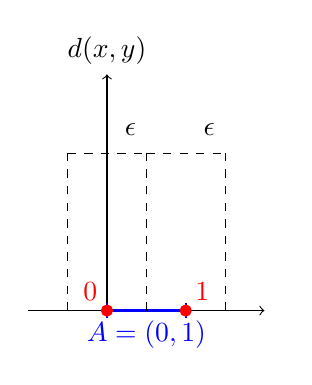
\begin{tikzpicture}
        % Draw the axes
        \draw[->] (-1, 0) -- (2, 0) node[right] {$\R$};
        \draw[->] (0, 0) -- (0, 3) node[above] {$d(x, y)$};

        % Draw the set A = (0, 1)
        \draw[thick, blue] (0, 0) -- (1, 0);
        \draw[thick, blue] (0, 0.1) -- (0, -0.1);
        \draw[thick, blue] (1, 0.1) -- (1, -0.1);
        \node[blue] at (0.5, -0.3) {$A = (0, 1)$};

        % Draw the limit points
        \filldraw[red] (0, 0) circle (2pt) node[above left] {$0$};
        \filldraw[red] (1, 0) circle (2pt) node[above right] {$1$};

        % Draw the epsilon radius for limit point 0
        \draw[dashed] (-0.5, 0) -- (-0.5, 2);
        \draw[dashed] (0.5, 0) -- (0.5, 2);
        \draw[dashed] (-0.5, 2) -- (0.5, 2);
        \node at (0.3, 2.3) {$\epsilon$};

        % Draw the epsilon radius for limit point 1
        \draw[dashed] (0.5, 0) -- (0.5, 2);
        \draw[dashed] (1.5, 0) -- (1.5, 2);
        \draw[dashed] (0.5, 2) -- (1.5, 2);
        \node at (1.3, 2.3) {$\epsilon$};
    \end{tikzpicture}
    \caption{Limit Points of the set $A = (0, 1)$ on the real line [Absolute Value Metric]}
\end{figure}
\begin{mydefinition}{Closed Set}
    Let $(X, d)$ be a metric space and $A \subseteq X$. The set $A$ is called a \underemphasise{closed set} if the set contains all its limit points. That is:
    $$\text{If } x \text{ is a limit point of } A, \text{ then } x \in A$$
\end{mydefinition}
\begin{mytheorem}[Complement of an Open Set is Closed and vice versa]
    Let $(X, d)$ be a metric space and $A \subseteq X$. Then, the set $A$ is closed if and only if its complement $X \backslash A$ is an open set.
\end{mytheorem}
\begin{proof}
    $(\Rightarrow)$ Assume that $A$ is a closed set. We need to show that $X \backslash A$ is an open set. Let $x \in X \backslash A$. Since $x \notin A$ and $A$ is closed, $x$ is not a limit point of $A$. Therefore, there exists a neighborhood $N(x, \epsilon)$ of $x$ such that:
    $$N(x, \epsilon) \cap A = \phi$$
    This implies that:
    $$N(x, \epsilon) \subseteq X \backslash A$$
    Hence, every point in $X \backslash A$ is an interior point of $X \backslash A$. Therefore, $X \backslash A$ is an open set. \\
    $(\Leftarrow)$ Assume that $X \backslash A$ is an open set. We need to show that $A$ is a closed set. Let $x$ be a limit point of $A$. We need to show that $x \in A$. Assume, for the sake of contradiction, that $x \notin A$. Then, $x \in X \backslash A$. Since $X \backslash A$ is an open set, there exists a neighborhood $N(x, \epsilon)$ of $x$ such that:
    $$N(x, \epsilon) \subseteq X \backslash A$$
    This implies that:
    $$N(x, \epsilon) \cap A = \phi$$
    which contradicts the fact that $x$ is a limit point of $A$. Hence, our assumption that $x \notin A$ is false. Therefore, $x \in A$. Thus, we have shown that if $x$ is a limit point of $A$, then $x \in A$. Hence, $A$ is a closed set.
\end{proof}
\begin{example}
    In the metric space $(\R, d)$ where $d(x, y) = |x - y|$ for all $x, y \in \R$, the set $A = [0, 1]$ is a closed set. This is because its complement $\R \backslash A = (-\infty, 0) \cup (1, \infty)$ is an open set. Both $(-\infty, 0)$ and $(1, \infty)$ are open intervals, and the union of open sets is also an open set. Hence, $A$ is a closed set.
\end{example}
\begin{example}
    In the metric space $(\R, d)$ where $d(x, y) = |x - y|$ for all $x, y \in \R$, the set $A = (0, 1)$ is not a closed set. This is because its complement $\R \backslash A = (-\infty, 0] \cup [1, \infty)$ is not an open set. The points $0$ and $1$ are limit points of $A$ but they are not included in $A$. Hence, $A$ does not contain all its limit points and is therefore not a closed set.
\end{example}
\begin{mytheorem}[All subsets of a discrete metric space are closed]
    Let $(X, d)$ be a metric space where $d$ is the discrete metric defined as:
    $$d(x, y) = 
    \begin{cases}
        0 & \text{if } x = y \\
        1 & \text{if } x \neq y
    \end{cases}$$
    Then, every subset of $X$ is a closed set.
\end{mytheorem}
\begin{proof}
    Let $A \subseteq X$ be any subset of $X$. We need to show that $A$ contains all its limit points. Let $x$ be a limit point of $A$. We need to show that $x \in A$. Assume, for the sake of contradiction, that $x \notin A$. Then, $x \in X \backslash A$. Since $X \backslash A$ is an open set (by the previous theorem), there exists a neighborhood $N(x, \epsilon)$ of $x$ such that:
    $$N(x, \epsilon) \subseteq X \backslash A$$
    We can choose $\epsilon = 0.5$. The neighborhood of $x$ is given by:
    $$N(x, 0.5) = \{y \in X: d(x, y) < 0.5\} = \{x\}$$
    since the only point that satisfies $d(x, y) < 0.5$ is $y = x$. Therefore, we have:
    $$N(x, 0.5) = \{x\} \subseteq X \backslash A$$
    This implies that:
    $$N(x, 0.5) \cap A = \phi$$
    which contradicts the fact that $x$ is a limit point of $A$. Hence, our assumption that $x \notin A$ is false. Therefore, $x \in A$. Thus, we have shown that if $x$ is a limit point of $A$, then $x \in A$. Hence, $A$ is a closed set.
\end{proof}
\begin{mydefinition}{Clopen Set}
    A set that is both an open set and a closed set is called a \underemphasise{clopen set}.
\end{mydefinition}
\begin{mytheorem}[All metric spaces are Clopen]
    Let $(X, d)$ be a metric space. Then, the set $X$ is both an open set and a closed set.
\end{mytheorem}
\begin{proof}
    To show that $X$ is an open set, let $x \in X$. We can choose any $\epsilon > 0$. The neighborhood of $x$ is given by:
    $$N(x, \epsilon) = \{y \in X: d(x, y) < \epsilon\}$$
    Since $N(x, \epsilon) \subseteq X$ for any $\epsilon > 0$, we have:
    $$N(x, \epsilon) \subseteq X$$
    Hence, every point in $X$ is an interior point of $X$. Therefore, $X$ is an open set. \\
    To show that $X$ is a closed set, let $x$ be a limit point of $X$. We need to show that $x \in X$. Since $x$ is a limit point of $X$, for every neighborhood $N(x, \epsilon)$ of $x$, we have:
    $$N(x, \epsilon) \cap X \neq \phi$$
    This implies that there exists some point $y \in N(x, \epsilon)$ such that $y \in X$. Since $y \in X$ and $X$ is the entire metric space, we have:
    $$x = y \in X$$
    Thus, we have shown that if $x$ is a limit point of $X$, then $x \in X$. Hence, $X$ is a closed set.
\end{proof}
\section{Perfect Sets and Compact Sets}
\subsection{Perfect Sets}
\begin{mydefinition}{Perfect Set}
    Let $(X, d)$ be a metric space and $A \subseteq X$. The set $A$ is called a \underemphasise{perfect set} if $A$ is closed and every point in $A$ is a limit point of $A$. That is:
    \begin{enumerate}
        \item $A$ is a closed set.
        \item $\forall x \in A, \forall \epsilon > 0: N(x, \epsilon) \cap (A \backslash \{x\}) \neq \phi$
    \end{enumerate}
    Intuitively, a perfect set is a set that is "complete" in the sense that it contains all its limit points and every point in the set can be "approached" by other points in the set.
\end{mydefinition}
\begin{example}
    In the metric space $(\R, d)$ where $d(x, y) = |x - y|$ for all $x, y \in \R$, the set $A = [0, 1]$ is not a perfect set. This is because the points $0$ and $1$ are not limit points of $A$. For example, let $x = 0$. For any $\epsilon > 0$, the neighborhood of $x$ is given by:
    $$N(0, \epsilon) = (-\epsilon, \epsilon)$$
    This neighborhood will always contain points that are not in $A$, such as $-0.5$ or $0.5$. Hence, there does not exist a neighborhood of $0$ that intersects with $A \backslash \{0\}$. Similarly, this can be shown for the point $1$. Therefore, not every point in $A$ is a limit point of $A$. Hence, $A$ is not a perfect set.
\end{example}
\begin{example}
    An example of a perfect set in $\R$ is the closed interval $[0, 1]$ with the endpoints removed, i.e., $(0, 1)$. This set is closed because it contains all its limit points (which are all the points in the interval). Additionally, every point in $(0, 1)$ is a limit point of the set since for any point $x \in (0, 1)$ and any $\epsilon > 0$, the neighborhood $N(x, \epsilon)$ will always contain other points from the set. Hence, $(0, 1)$ is a perfect set.
\end{example}
\begin{mytheorem}
    Let $(X, d)$ be a metric space and $A \subseteq X$. If $A$ is a perfect set, then $A$ is uncountable.
\end{mytheorem}
\begin{proof}
    Assume, for the sake of contradiction, that $A$ is a perfect set and $A$ is at most countable. Then, we can list the elements of $A$ as $\{x_1, x_2, x_3, ...\}$. Since $A$ is a perfect set, every point in $A$ is a limit point of $A$. Therefore, for each $x_n \in A$, there exists a neighborhood $N(x_n, \epsilon_n)$ such that:
    $$N(x_n, \epsilon_n) \cap (A \backslash \{x_n\}) \neq \phi$$
    We can choose $\epsilon_n$ such that $N(x_n, \epsilon_n)$ are disjoint for different $n$. This is possible because we can choose $\epsilon_n$ to be small enough such that the neighborhoods do not overlap. \\
    Now, consider the set $B = \bigcup_{n=1}^{\infty} N(x_n, \epsilon_n)$. Since the neighborhoods are disjoint, we have:
    $$B \cap A = \bigcup_{n=1}^{\infty} (N(x_n, \epsilon_n) \cap A)$$
    Since each $N(x_n, \epsilon_n) \cap A$ is non-empty, we have that $B \cap A$ is also non-empty. However, this contradicts the fact that $A$ is at most countable, as we have constructed an uncountable set $B \cap A$. \\ 
    Hence, our assumption that $A$ is at most countable is false. Therefore, $A$ is uncountable.
\end{proof}
\subsection{Compact Sets}
\begin{mydefinition}{Open Cover}
    Let $(X, d)$ be a metric space and $A \subseteq X$. An \underemphasise{open cover} of $A$ is a collection of open sets $\{U_i\}_{i \in I}$ where $I$ is an index set such that:
    $$A \subseteq \bigcup_{i \in I} U_i$$
    Intuitively, an open cover is a collection of open sets that "cover" the set $A$.
\end{mydefinition}
\begin{example}
    In the metric space $(\R, d)$ where $d(x, y) = |x - y|$ for all $x, y \in \R$, let $A = [0, 1]$. An example of an open cover of $A$ is given by the collection of open intervals:
    $$\{(-1, 0.5), (0.4, 0.6), (0.5, 1.5)\}$$
    We can see that:
    $$[0, 1] \subseteq (-1, 0.5) \cup (0.4, 0.6) \cup (0.5, 1.5)$$
    Hence, the collection $\{(-1, 0.5), (0.4, 0.6), (0.5, 1.5)\}$ is an open cover of $A$.
\end{example}
\begin{mydefinition}{Finite Subcover}
    Let $(X, d)$ be a metric space and $A \subseteq X$. A \underemphasise{finite subcover} of an open cover $\{U_i\}_{i \in I}$ of $A$ is a finite collection of open sets $\{U_{i_1}, U_{i_2}, ..., U_{i_n}\}$ such that:
    $$A \subseteq \bigcup_{k=1}^{n} U_{i_k}$$
    Intuitively, a finite subcover is a finite collection of open sets from the original open cover that still "covers" the set $A$.
\end{mydefinition}
\begin{example}
    In the metric space $(\R, d)$ where $d(x, y) = |x - y|$ for all $x, y \in \R$, let $A = [0, 1]$. Consider the open cover of $A$ given by the collection of open intervals:
    $$\{(-1, 0.5), (0.4, 0.6), (0.5, 1.5)\}$$
    A finite subcover of this open cover is given by the collection of open intervals:
    $$\{(-1, 0.5), (0.5, 1.5)\}$$
    We can see that:
    $$[0, 1] \subseteq (-1, 0.5) \cup (0.5, 1.5)$$
    Hence, the collection $\{(-1, 0.5), (0.5, 1.5)\}$ is a finite subcover of the original open cover.
\end{example}
\begin{mydefinition}{Compact Set}
    Let $(X, d)$ be a metric space and $A \subseteq X$. The set $A$ is called a \underemphasise{compact set} if every open cover of $A$ has a finite subcover. That is:
    $$\text{For every open cover } \{U_i\}_{i \in I} \text{ of } A, \exists \{U_{i_1}, U_{i_2}, ..., U_{i_n}\} \text{ such that } A \subseteq \bigcup_{k=1}^{n} U_{i_k}$$
    Intuitively, a compact set is a set that can be "covered" by a finite number of open sets from any open cover.
\end{mydefinition}
\begin{mynote}
\underemphasise{Why are compact sets important?} Compact sets are important in analysis and topology because they have several useful properties. For example, every continuous function defined on a compact set is bounded and attains its maximum and minimum values. Additionally, compact sets are closed and bounded in $\R^n$, which makes them easier to work with in many mathematical contexts. Compactness is also a key concept in various theorems, such as the Heine-Borel theorem and the Arzelà-Ascoli theorem.
\end{mynote}
\begin{example}
    In the metric space $(\R, d)$ where $d(x, y) = |x - y|$ for all $x, y \in \R$, the set $A = [0, 1]$ is a compact set. This is because every open cover of $A$ has a finite subcover. For example, consider the open cover of $A$ given by the collection of open intervals:
    $$\{(-1, 0.5), (0.4, 0.6), (0.5, 1.5)\}$$
    A finite subcover of this open cover is given by the collection of open intervals:
    $$\{(-1, 0.5), (0.5, 1.5)\}$$
    We can see that:
    $$[0, 1] \subseteq (-1, 0.5) \cup (0.5, 1.5)$$
    Hence, the collection $\{(-1, 0.5), (0.5, 1.5)\}$ is a finite subcover of the original open cover. This can be shown for any open cover of $A$, hence $A$ is a compact set.
\end{example}
\subsection{Heine-Borel Theorem on Compact Sets in $\R^n$}
It is significantly easier to determine whether a set is closed and bounded than to check if every open cover has a finite subcover. The Heine-Borel theorem provides a useful characterization of compact sets in $\R^n$, making it easier to identify compact sets in this context. We can use this theorem to determine whether a set is compact by simply checking if it is closed and bounded.
\begin{mytheorem}[Heine-Borel Theorem A]
    A subset $A$ of $\R^n$ is closed and bounded if it is compact.
\end{mytheorem}
\begin{proof}
    Let $A \subseteq \R^n$ be a compact set. We need to show that $A$ is closed and bounded. \\
    To show that $A$ is bounded, we can consider the open cover of $A$ given by the collection of open balls:
    $$\{B(x, 1) : x \in A\}$$
    Since $A$ is compact, there exists a finite subcover of this open cover. Let $\{B(x_1, 1), B(x_2, 1), ..., B(x_m, 1)\}$ be the finite subcover. Then, we have:
    $$A \subseteq \bigcup_{i=1}^{m} B(x_i, 1)$$
    This implies that for any point $y \in A$, there exists some $i$ such that $y \in B(x_i, 1)$. Therefore, we have:
    $$d(y, x_i) < 1$$
    for some $i = 1, 2, ..., m$. This implies that:
    $$d(y, 0) \leq d(y, x_i) + d(x_i, 0) < 1 + d(x_i, 0)$$
    Since there are only finitely many $x_i$, we can let $M = \max\{d(x_i, 0) : i = 1, 2, ..., m\}$. Then, we have:
    $$d(y, 0) < 1 + M$$
    for all $y \in A$. Hence, $A$ is bounded. \\
    To show that $A$ is closed, let $x$ be a limit point of $A$. We need to show that $x \in A$. Assume, for the sake of contradiction, that $x \notin A$. Then, $x \in \R^n \backslash A$. Since $\R^n \backslash A$ is an open set (by the previous theorem), there exists a neighborhood $N(x, \epsilon)$ of $x$ such that:
    $$N(x, \epsilon) \subseteq \R^n \backslash A$$
    This implies that:
    $$N(x, \epsilon) \cap A = \phi$$
    which contradicts the fact that $x$ is a limit point of $A$. Hence, our assumption that $x \notin A$ is false. Therefore, $x \in A$. Thus, we have shown that if $x$ is a limit point of $A$, then $x \in A$. Hence, $A$ is a closed set. \\
    Therefore, we conclude that if $A$ is a compact set in $\R^n$, then $A$ is closed and bounded.
\end{proof}
\begin{mytheorem}[Heine-Borel Theorem B]
    A subset $A$ of $\R^n$ is compact if it is closed and bounded.
\end{mytheorem}
\begin{proof}
    Let $A \subseteq \R^n$ be a closed and bounded set. We need to show that $A$ is compact. \\
    Since $A$ is bounded, there exists some $M > 0$ such that:
    $$A \subseteq B(0, M)$$
    where $B(0, M)$ is the open ball of radius $M$ centered at the origin. \\
    Let $\{U_i\}_{i \in I}$ be an open cover of $A$. Since $B(0, M)$ is an open set, we can consider the open cover of $B(0, M)$ given by the collection of open balls:
    $$\{B(x, r) : x \in B(0, M), r > 0\}$$
    Since $B(0, M)$ is an open set in $\R^n$, it is also a compact set (by the previous theorem). Therefore, there exists a finite subcover of this open cover. Let $\{B(x_1, r_1), B(x_2, r_2), ..., B(x_m, r_m)\}$ be the finite subcover. Then, we have:
    $$B(0, M) \subseteq \bigcup_{i=1}^{m} B(x_i, r_i)$$
    This implies that for any point $y \in A$, there exists some $i$ such that $y \in B(x_i, r_i)$. Therefore, we have:
    $$d(y, x_i) < r_i$$
    for some $i = 1, 2, ..., m$. This implies that:
    $$d(y, 0) \leq d(y, x_i) + d(x_i, 0) < r_i + d(x_i, 0)$$
    Since there are only finitely many $x_i$, we can let $N = \max\{r_i + d(x_i, 0) : i = 1, 2, ..., m\}$. Then, we have:
    $$d(y, 0) < N$$
    for all $y \in A$. Hence, $A$ is bounded. \\
    To show that $A$ is closed, let $x$ be a limit point of $A$. We need to show that $x \in A$. Assume, for the sake of contradiction, that $x \notin A$. Then, $x \in \R^n \backslash A$. Since $\R^n \backslash A$ is an open set (by the previous theorem), there exists a neighborhood $N(x, \epsilon)$ of $x$ such that:
    $$N(x, \epsilon) \subseteq \R^n \backslash A$$
    This implies that:
    $$N(x, \epsilon) \cap A = \phi$$
    which contradicts the fact that $x$ is a limit point of $A$. Hence, our assumption that $x \notin A$ is false. Therefore, $x \in A$. Thus, we have shown that if $x$ is a limit point of $A$, then $x \in A$. Hence, $A$ is a closed set. \\
    Therefore, we conclude that if $A$ is a closed and bounded set in $\R^n$, then $A$ is compact.
\end{proof}
\chapter{Sequences and Series}
All undefined terms have their usual meanings. 
\section{Sequences}
\subsection{Sequences and their limits}
\begin{mydefinition}{Sequences and Terms}
    A \underemphasise{sequence} in a set $S$ is a function: $f: \N \rightarrow A$ where $A \subseteq S$. \\ 
    The value of this function $f$ at any fixed $n \in \N$ is denoted by $x_n$ and is referred to as the  $n^{th}$ \underemphasise{term} of the sequence. Other letters can be used as identifiers for terms, such as $z, y$, etc. \\\\
    A sequence in $\R$ for example, is a function $f: \N \rightarrow A$, where $A \subseteq \R$ and the terms of the sequence are denoted by $x_n = f(n)$ for $n \in \N$. \\\\
    A sequence itself is denoted as $(x_n : n \in \N)$, this is different from the notation for a set, which is denoted as $\{x_n : n \in \N\}$. The former denotes a sequence, while the latter denotes a set of terms (the difference is that a sequence has an ordering, while a set does not). 
\end{mydefinition}
\begin{example}
    Consider the sequence $(x_n : n \in \N)$ in $\R$ defined by the function $f: \N \rightarrow \R$ where $f(n) = \frac{1}{n}$ for all $n \in \N$. The terms of this sequence are given by:
    $$x_1 = f(1) = 1$$
    $$x_2 = f(2) = \frac{1}{2}$$
    $$x_3 = f(3) = \frac{1}{3}$$
    $$\vdots$$
    $$x_n = f(n) = \frac{1}{n}$$
    Thus, the sequence can be written as:
    $$(x_n : n \in \N) = \left(1, \frac{1}{2}, \frac{1}{3}, \frac{1}{4}, ...\right)$$
    \begin{figure}[H]
        \centering
        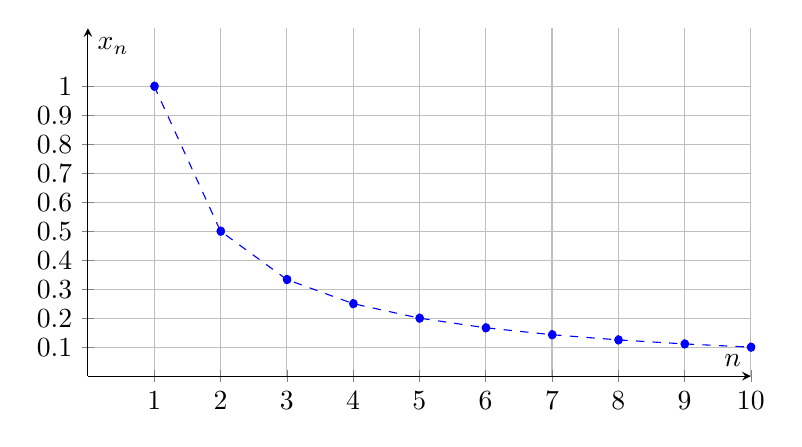
\begin{tikzpicture}
        \begin{axis}[
            axis lines = middle,
            xlabel = $n$,
            ylabel = {$x_n$},
            ymin=0, ymax=1.2,
            xmin=0, xmax=10,
            xtick={1,2,3,4,5,6,7,8,9,10},
            ytick={0.1,0.2,0.3,0.4,0.5,0.6,0.7,0.8,0.9,1.0},
            grid = both,
            width=10cm,
            height=6cm
        ]
        \addplot[
            dashed,
            mark=*,
            mark size=1.5pt,
            color=blue
        ] coordinates {
            (1, 1)
            (2, 0.5)
            (3, 0.3333)
            (4, 0.25)
            (5, 0.2)
            (6, 0.1667)
            (7, 0.1429)
            (8, 0.125)
            (9, 0.1111)
            (10, 0.1)
        };
        \end{axis}
        \end{tikzpicture}
        \caption{The sequence defined by $f(n) = \frac{1}{n}$}
    \end{figure}
\end{example}
\begin{mydefinition}{Limit of a Sequence and convergence/divergence}
    Let $(x_n : n \in \N)$ be a sequence in $\R$. We say that the sequence \underemphasise{converges} to a real number $L$ if:
    $$\forall \epsilon > 0, \exists N \in \N: n > N \implies |x_n - L| < \epsilon$$
    In this case, we write $\limit{n}{\infty}{x_n} = L$ or simply $\lim(x_n) = L$. If a sequence does not converge to any real number, we say that it is \underemphasise{divergent}. \\
    The number $L$ is called the \underemphasise{limit} of the sequence $(x_n : n \in \N)$.
\end{mydefinition}
\begin{mynote}
    Intuitively, the definition of convergence means that as $n$ becomes larger and larger, the terms of the sequence get arbitrarily close to the limit $L$. The number $N$ in the definition is a threshold beyond which all terms of the sequence are within $\epsilon$ distance from $L$. That just means that for any epsilon you can think of, for sufficiently large $n$, the terms of the sequence will be within that epsilon distance from $L$. The sufficiently large is defined by $N$.
\end{mynote}
\begin{mytheorem}[Uniqueness of Limits]
    If a sequence $(x_n : n \in \N)$ converges to two different limits $L_1$ and $L_2$, then $L_1 = L_2$.
\end{mytheorem}
\begin{proof}
    Assume that $(x_n : n \in \N)$ converges to two different limits $L_1$ and $L_2$. Then, by the definition of convergence, we have:
    $$\forall \epsilon > 0, \exists N_1 \in \N: n > N_1 \implies |x_n - L_1| < \epsilon$$
    $$\forall \epsilon > 0, \exists N_2 \in \N: n > N_2 \implies |x_n - L_2| < \epsilon$$
    Let $N = \max(N_1, N_2)$.
    By the triangle inequality, we have:
    $$\forall \epsilon > 0, n>N: |L_1 - L_2| = |(L_1 - x_n) + (x_n - L_2)| \leq |L_1 - x_n| + |x_n - L_2| < 2\epsilon$$ 
    $$\implies \abs{L_1 -L_2} = 0 \implies L_1 = L_2$$
    Hence, we conclude that if a sequence converges to two different limits, then those limits must be equal.
\end{proof}
\begin{mytheorem}[Presence of infinite terms within epsilon distance from the limit]
    If a sequence $(x_n : n \in \N)$ converges, then we can find a natural number $N$ such that for all $n > N$, the terms of the sequence are within a distance of $\epsilon$ from each other. That is:
    $$\forall \epsilon > 0, \exists N \in \N: m, n > N \implies |x_n - x_m| < \epsilon$$
\end{mytheorem}
\begin{proof}
    Let $(x_n : n \in \N)$ be a sequence that converges to $L$. Then, by the definition of convergence, we have:
    $$\forall \epsilon > 0, \exists N \in \N: m , n > N \implies |x_n - L| < \frac{\epsilon}{2} \nd |x_m - L| < \frac{\epsilon}{2}$$
    Then, by the triangle inequality, we have:
    $$|x_n - x_m| = |(x_n - L) + (L - x_m)| \leq |x_n - L| + |L - x_m| < \frac{\epsilon}{2} + \frac{\epsilon}{2} = \epsilon$$
    Hence, we conclude that for all $m, n > N$, the terms of the sequence are within a distance of $\epsilon$ from each other.
\end{proof}
\subsection{Limit Theorems}
\begin{mytheorem}[Limit Theorems for Sequences]
    Let $X = (x_n : n \in \N)$ and $Y = (y_n : n \in \N)$ be two sequences in $\R$ that converge to limits $L_1$ and $L_2$ respectively. Then, the following limit theorems hold:
    \begin{enumerate}
        \item If $x_n > 0, \forall n \in \N$, then $\limit{n}{\infty}{x_n} \geq 0$.
        \item If $x_n \geq y_n, \forall n \in \N$, then $L_1 \geq L_2$.
    \end{enumerate}
\end{mytheorem}
\begin{proof}
    We prove each part separately. \\
    \begin{enumerate}
        \item Assume, for the sake of contradiction, that $\limit{n}{\infty}{x_n} = L < 0$. Then, by the definition of convergence, we have:
        $$\forall \epsilon > 0, \exists N \in \N: n > N \implies |x_n - L| < \epsilon$$
        Let us take $\epsilon = \frac{-L}{2}$. Then, we have:
        $$\exists N \in \N: n > N \implies |x_n - L| < \frac{-L}{2}$$
        This implies that for all $n > N$, we have:
        $$x_n < L + \frac{-L}{2} = \frac{-L}{2} < 0$$
        This is a contradiction, as we assumed that $x_n > 0$ for all $n \in \N$. Hence, we conclude that $\limit{n}{\infty}{x_n} \geq 0$.
        \item Assume, for the sake of contradiction, that $L_1 < L_2$. Then, by the definition of convergence, we have:
        $$\forall \epsilon > 0, \exists N_1 \in \N: n > N_1 \implies |x_n - L_1| < \epsilon$$
        $$\forall \epsilon > 0, \exists N_2 \in \N: n > N_2 \implies |y_n - L_2| < \epsilon$$
        Let $\epsilon = \left|\frac{L_2 - L_1}{2}\right|$. Then, we have:
        $$\exists N_1 \in \N: n > N_1 \implies |x_n - L_1| < \left|\frac{L_2 - L_1}{2}\right|$$
        $$\exists N_2 \in \N: n > N_2 \implies |y_n - L_2| < \left|\frac{L_2 - L_1}{2}\right|$$
        Let $N = \max(N_1, N_2)$. Then, for all $n > N$, we have:
        $$x_n < L_1 + \left|\frac{L_2 - L_1}{2}\right| = \frac{L_1 + L_2}{2}$$
        $$y_n > L_2 - \left|\frac{L_2 - L_1}{2}\right| = \frac{L_1 + L_2}{2}$$
        This implies that for all $n > N$, we have:
        $$x_n < y_n$$
        This is a contradiction, as we assumed that $x_n \geq y_n$ for all $n \in \N$. Hence, we conclude that $L_1 \geq L_2$.
    \end{enumerate}
\end{proof}
\begin{mydefinition}{Bounded Sequences}
    A sequence $(x_n : n \in \N)$ is said to be \underemphasise{bounded above} if there exists a real number $\alpha$ such that:
    $$\forall n \in \N, x_n \leq \alpha$$
    Similarly, a sequence is said to be \underemphasise{bounded below} if there exists a real number $\beta$ such that:
    $$\forall n \in \N, x_n \geq \beta$$
    If a sequence is bounded above and below, we say that it is \underemphasise{bounded}.
\end{mydefinition}
\begin{figure}[H]
    \centering
    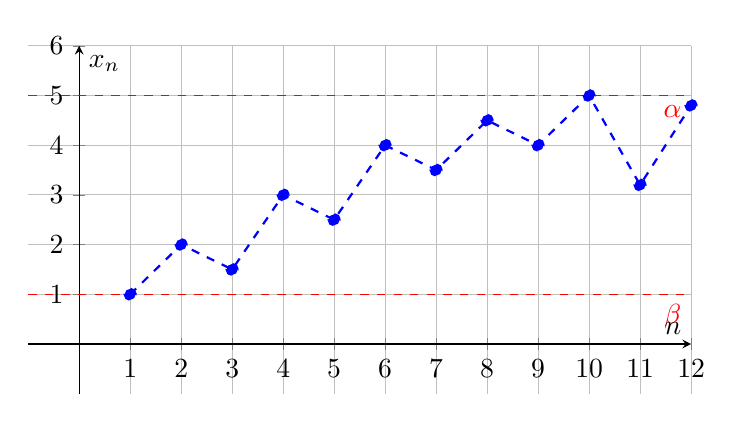
\begin{tikzpicture}
        \begin{axis}[
            axis lines = middle,
            xlabel = $n$,
            ylabel = {$x_n$},
            ymin = -1, ymax = 6,
            xmin = -1, xmax = 12,
            xtick={0,1,2,3,4,5,6,7,8,9,10,11,12},
            ytick={0,1,2,3,4,5,6},
            grid = both,
            width=10cm,
            height=6cm,
        ]
        \addplot[dashed, thick,
            color=blue,
            mark=*,
            mark options={fill=blue}
        ] coordinates {
            (1, 1)
            (2, 2)
            (3, 1.5)
            (4, 3)
            (5, 2.5)
            (6, 4)
            (7, 3.5)
            (8, 4.5)
            (9, 4)
            (10, 5)
            (11, 3.2)
            (12, 4.8)
        };
        \draw[dashed, red] (axis cs:-1,1) -- (axis cs:12,1) node[anchor=north east] {$\beta$};
        \draw[dashed, red] (axis cs:-1,5) -- (axis cs:12,5) node[anchor=north east] {$\alpha$};
        \end{axis}
    \end{tikzpicture}
    \caption{A bounded sequence with upper bound $\alpha$ and lower bound $\beta$}
    \label{fig:bounded_sequence}
\end{figure}
\begin{mytheorem}[Convergent Sequences are bounded]
    If a sequence $X = (x_n : n \in \N)$ converges, then it is bounded. 
\end{mytheorem}
\begin{proof}
    Let $X = (x_n : n \in \N)$ be a sequence that converges to $L$. Then, by the definition of convergence, we have:
    $$\forall \epsilon > 0, \exists N \in \N: n > N \implies |x_n - L| < \epsilon$$
    Let us take $\epsilon = 1$. Then, we have:
    $$\exists N \in \N: n > N \implies |x_n - L| < 1$$
    This implies that for all $n > N$, we have:
    $$x_n < L + 1$$
    Let $\alpha = \max\{L + 1, x_1, x_2, \ldots, x_N\}$. 
    Then, we have:
    $$\forall n \in \N, x_n \leq \alpha$$
    We also know that for $n > N$, all terms of the sequence are within a distance of 1 from $L$. Therefore, we have:
    $$\forall n> N: x_n > L - 1$$
    Let $\beta = \min\{L - 1, x_1, x_2, \ldots, x_N\}$. 
    Then, we have:
    $$\forall n \in \N, x_n \geq\beta$$
    Therefore, we have shown that the sequence $X = (x_n : n \in \N)$ is bounded above by $\alpha$ and below by $\beta$. Hence, we conclude that convergent sequences are bounded.
\end{proof}
\begin{mynote}
    The definition of convergence is useful only to verify that a sequence converges to a limit. It is not useful to find the limit of a sequence. It does not provide an algorithm to find the limit. 
\end{mynote}
\begin{mydefinition}{Tail of a Sequence}
    The \underemphasise{tail} of a sequence $(x_n : n \in \N)$ is the sequence $(x_n : n \geq N)$ for some fixed $N \in \N$. \\
    In general, we can define the $m^{th}$ tail of a sequence $(x_n : n \in \N)$ as the sequence $(x_{m+n} : n \in \N)$.
\end{mydefinition}
\begin{mytheorem}[Convergence of Tails]
    If and only if a sequence $(x_n : n \in \N)$ converges to $L$, then all its tails converge to $L$. 
\end{mytheorem}
\begin{proof}
    The $p^{th}$ term of the $m^{th}$ tail of a sequence $(x_n : n \in \N)$ is $x_{m+p}$ or the $(m+p)^{th}$ term of the original sequence. 
    By the definition of convergence, we have:
    $$\forall \epsilon > 0, \exists N \in \N: n > N \implies |x_n - L| < \epsilon$$
    If $N< m$, then the above definition holds for all $m^{th}$ tails by definition. 
    If $N \geq m$, then we can take $N' = N - m$. Then, we have:
    $$\forall \epsilon > 0, \exists N' \in \N: n > N' \implies |x_{m+n} - L| < \epsilon$$
    Hence, we conclude that all tails of a convergent sequence converge to the same limit.
    Conversely, if all tails of a sequence converge to $L$, then by the definition of convergence, we have:
    $$\forall \epsilon > 0, \exists N \in \N: n > N \implies |x_{m+n} - L| < \epsilon$$
    Let $N' = N + m$. Then, we have:
    $$\forall \epsilon > 0, \exists N' \in \N: n > N' \implies |x_n - L| < \epsilon$$
    Hence, we conclude that the sequence converges to $L$.
\end{proof}
\begin{mydefinition}{Ultimate Properties}
    A sequence $(x_n : n \in \N)$ ultimately has a property if there exists a tail of the sequence that has the property.
\end{mydefinition}
\begin{mytheorem}[Algebra of Limits]
    Let $(x_n : n \in \N)$ and $(y_n : n \in \N)$ be two sequences in $\R$ that converge to $L_x$ and $L_y$ respectively. Then, we have the following results:
    \begin{enumerate}
        \item $\limit{n}{\infty}{(x_n + y_n)} = L_x + L_y$
        \item $\limit{n}{\infty}{(cx_n)} = c L_x$ for any $c \in \R$
        \item $\limit{n}{\infty}{(x_n y_n)} = L_x L_y$
    \end{enumerate}
\end{mytheorem}
\begin{proof}
    We prove all the results using the Triangle Inequality. 
    \begin{enumerate}
    \item Let $\epsilon > 0$. Then, by the definition of convergence, we have:
    $$\exists N_x \in \N: n > N_x \implies |x_n - L_x| < \frac{\epsilon}{2}$$
    $$\exists N_y \in \N: n > N_y \implies |y_n - L_y| < \frac{\epsilon}{2}$$
    Let $N = \max(N_x, N_y)$. Then, we have:
    $$\forall n > N: |(x_n + y_n) - (L_x + L_y)| = |(x_n - L_x) + (y_n - L_y)| \leq |x_n - L_x| + |y_n - L_y| < \frac{\epsilon}{2} + \frac{\epsilon}{2} = \epsilon$$
    Hence, we conclude that $\limit{n}{\infty}{(x_n + y_n)} = L_x + L_y$. \\
    \item Let $\epsilon > 0$. Then, by the definition of convergence, we have:
    $$\exists N_x \in \N: n > N_x \implies |x_n - L_x| < \frac{\epsilon}{|c|}$$
    Then, we have:  
    $$\forall n > N_x: |cx_n - cL_x| = |c(x_n - L_x)| = |c||x_n - L_x| < |c|\frac{\epsilon}{|c|} = \epsilon$$
    Hence, we conclude that $\limit{n}{\infty}{(cx_n)} = c L_x$. \\
    \item Let $\epsilon > 0$. Then, by the definition of convergence, we have:
    $$\exists N_x \in \N: n > N_x \implies |x_n - L_x| < \epsilon$$
    $$\exists N_y \in \N: n > N_y \implies |y_n - L_y| < \epsilon$$
    Consider: 
    $$\abs{x_n y_n - L_x L_y} = \abs{(x_n - L_x)L_y + L_x(y_n - L_y)}$$
    By the triangle inequality, we have:
    $$\abs{x_n y_n - L_x L_y} \leq |y_n||x_n - L_x| + |L_x||y_n - L_y|$$
    Since $y_n$ converges, we can find a real number $M$ such that it is bounded by $M$. That is: 
    $$\exists M \in \R: \forall n \in \N, |y_n| \leq M$$
    Also, since $x_n$ converges, we can find a real number $N_x$ such that:
    $$\forall n > N_x, |x_n - L_x| < \frac{\epsilon}{2M}$$
    \begin{enumerate}
        \item \textbf{Case 1: $L_x = 0$}: In this case, we have:
        $$\abs{x_n y_n - L_x L_y} = \abs{L_y}\abs{(x_n - L_x)} < \frac{\epsilon}{2} < \epsilon$$
        \item \textbf{Case 2: $L_x \neq 0$}: Since $y_n$ converges, we can find a real number $N_y$ such that:
        $$\forall n > N_y, |y_n - L_y| < \frac{\epsilon}{2|L_x|}$$
        Then we have:
        $$\abs{x_n y_n - L_x L_y} < M\frac{\epsilon}{2M} + |L_x|\frac{\epsilon}{2|L_x|} = \frac{\epsilon}{2} + \frac{\epsilon}{2} = \epsilon$$
    \end{enumerate}
    \end{enumerate}
\end{proof}
\begin{mytheorem}[Squeeze Theorem or The Sandwich Theorem]
    Let $(x_n : n \in \N)$, $(y_n : n \in \N)$ and $(z_n : n \in \N)$ be three sequences in $\R$ such that:
    $$x_n \leq y_n \leq z_n$$
    for all $n > N$ for some $N \in \N$. If $\limit{n}{\infty}{x_n} = L$ and $\limit{n}{\infty}{z_n} = L$, then $\limit{n}{\infty}{y_n} = L$, that is: 
    $$(\exists N \in \N: n > N \implies x_n \leq y_n \leq z_n) \nd (\limit{n}{\infty}{x_n} = L \nd \limit{n}{\infty}{z_n} = L) \implies \exists \limit{n}{\infty}{y_n} \in \R : \limit{n}{\infty}{y_n} = L$$
\end{mytheorem}
\begin{proof}
    Let $\epsilon > 0$. Let $K$ be the natural number such that: 
    $$\forall n > K: x_n \leq y_n \leq z_n$$
    Then, by the definition of convergence, we have:
    $$\exists N_x \in \N: n > N_x \implies |x_n - L| < \epsilon$$
    $$\exists N_z \in \N: n > N_z \implies |z_n - L| < \epsilon$$
    Let $N = \max(N_x, N_z, K)$. Then, we have:
    $$\forall n > N: |x_n - L| < \epsilon \nd |z_n - L| < \epsilon$$
    Since $x_n \leq y_n \leq z_n$, we have:
    $$L - \epsilon < x_n \leq y_n \leq z_n < L + \epsilon$$
    Hence, we conclude that:
    $$|y_n - L| < \epsilon$$
    Therefore, we have shown that $\limit{n}{\infty}{y_n} = L$.
\end{proof}
\begin{mytheorem}[Inequality of Limits]
    Let $(x_n : n \in \N)$ and $(y_n : n \in \N)$ be two sequences in $\R$ that converge to $L_x$ and $L_y$ respectively. If $x_n \leq y_n$ for all $n \in \N$, then $L_x \leq L_y$.
\end{mytheorem}
\begin{proof}
    Let $z_n = y_n - x_n$. Then, we have:
    $$\forall n \in \N, z_n \geq 0$$
    Since $z_n$ is a sequence of non-negative real numbers, we know that it is bounded below by 0. By the algebra of limits, we have:
    $$\limit{n}{\infty}{z_n} = \limit{n}{\infty}{(y_n - x_n)} = L_y - L_x$$
    Since $z_n \geq 0$ for all $n \in \N$, we have:
    $$L_y - L_x \geq 0 \implies L_y \geq L_x$$
    Hence, we conclude that if $x_n \leq y_n$ for all $n \in \N$, then $L_x \leq L_y$.
\end{proof}
\begin{mytheorem}[Ratio test for convergence]
    Let $(x_n : n \in \N)$ be a sequence in $\R$ such that $x_n > 0$ for all $n \in \N$. If the limit of the sequence of ratios $\frac{x_{n+1}}{x_n}$ exists and is less than 1, then the sequence converges to 0. That is:
    $$\limit{n}{\infty}{\frac{x_{n+1}}{x_n}} = L < 1 \implies \limit{n}{\infty}{x_n} = 0$$
\end{mytheorem}
\begin{proof}
    By the theorem proved above, we can say that limit of the sequence of ratios $\limit{n}{\infty}{\frac{x_{n+1}}{x_n}} \geq 0$. \\
    Let $r$ be a number such that: $$L < r < 1$$
    Let $\epsilon = r-L > 0$. Then, by the definition of convergence, we have:
    $$\exists N \in \N: n > N \implies \left|\frac{x_{n+1}}{x_n} - L\right| < \epsilon$$
    Now we can write:
    $$\forall n > N: \frac{x_{n+1}}{x_n} < L + \epsilon = r$$
    Therefore, if we take $n > N$, we have:
    $$\frac{x_{n+1}}{x_n} < r \implies x_{n+1} < r x_n < x_{n-1}r^2 ... x_N r^{n - N +1}$$
    Set $C = \frac{x_N}{r^N}$. Then, we have:
    $$0< x_{n+1} < C r^{n+1}$$
    Now, since $r < 1$, we know that $r^{n+1} \rightarrow 0$ as $n \rightarrow \infty$ (see exercises for proof). Therefore, by the sandwich theorem we have:
    $$\lim_{n \to \infty} C r^{n+1} = C \cdot 0 = 0$$
    Hence, we conclude that $\limit{n}{\infty}{x_n} = 0$. 
\end{proof}
\subsection{Monotonic Sequences}
\begin{mydefinition}{Monotonic Sequences, Increasing and Decreasing Sequences}
    A sequence is monotonic if it is either increasing or decreasing. \\
    A sequence $(x_n : n \in \N)$ is said to be \underemphasise{increasing} if:
    $$\forall n \in \N, x_n \leq x_{n+1}$$
    A sequence $(x_n : n \in \N)$ is said to be \underemphasise{decreasing} if:
    $$\forall n \in \N, x_n \geq x_{n+1}$$
    A sequence is said to be \underemphasise{strictly increasing} if:
    $$\forall n \in \N, x_n < x_{n+1}$$
    A sequence is said to be \underemphasise{strictly decreasing} if:
    $$\forall n \in \N, x_n > x_{n+1}$$ 
\end{mydefinition}
\begin{figure}[H]
    \centering
    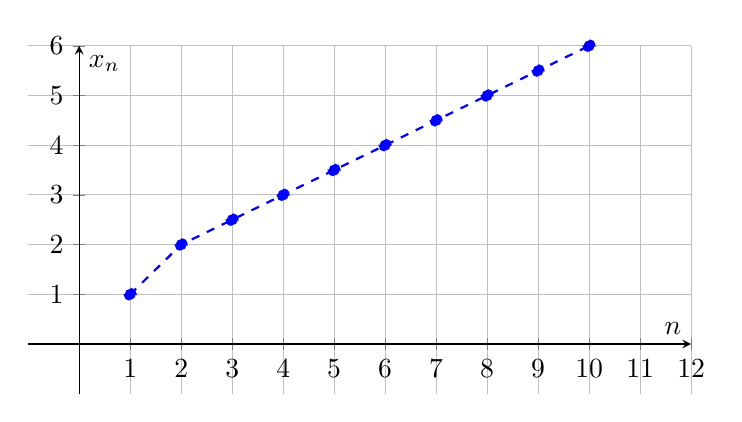
\begin{tikzpicture}
        \begin{axis}[
            axis lines = middle,
            xlabel = $n$,
            ylabel = {$x_n$},
            ymin = -1, ymax = 6,
            xmin = -1, xmax = 12,
            xtick={0,1,2,3,4,5,6,7,8,9,10,11,12},
            ytick={0,1,2,3,4,5,6},
            grid = both,
            width=10cm,
            height=6cm,
        ]
        \addplot[dashed, thick,
            color=blue,
            mark=*,
            mark options={fill=blue}
        ] coordinates {
            (1, 1)
            (2, 2)
            (3, 2.5)
            (4, 3)
            (5, 3.5)
            (6, 4)
            (7, 4.5)
            (8, 5)
            (9, 5.5)
            (10, 6)
        };
        \end{axis}
    \end{tikzpicture}
    \caption{An increasing sequence}
    \label{fig:increasing_sequence}
\end{figure}
\begin{mytheorem}[Bounded Monotonic Sequences are convergent]
    If a sequence $(x_n : n \in \N)$ is increasing and bounded above, then it converges to its supremum. Similarly, if a sequence $(x_n : n \in \N)$ is decreasing and bounded below, then it converges to its infimum. A monotone sequence converges if and only if it is bounded.
\end{mytheorem}
\begin{proof}
    We prove both parts seperately. \\
    $(\Rightarrow)$ Suppose $(x_n : n \in \N)$ is an increasing sequence that is bounded above. Let $L = \sup\{x_n : n \in \N\}$. We need to show that $\limit{n}{\infty}{x_n} = L$. \\
    Suppose, for the sake of contradiction, that $\limit{n}{\infty}{x_n} \neq L$. Then, by the definition of convergence, we have:
    $$\exists \epsilon > 0: \forall N \in \N, \exists n > N: |x_n - L| \geq \epsilon$$
    This implies that:
    $$\exists \epsilon > 0: \forall N \in \N, \exists n > N: x_n \leq L - \epsilon$$
    Since $L - \epsilon < L$, this contradicts the fact that $L$ is the least upper bound of the set $\{x_n : n \in \N\}$. Hence, our assumption that $\limit{n}{\infty}{x_n} \neq L$ is false. Therefore, we have $\limit{n}{\infty}{x_n} = L$. \\
    Similarly, we can prove that if a sequence $(x_n : n \in \N)$ is decreasing and bounded below, then it converges to its infimum. \\
    $(\Leftarrow)$ Let $x_n$ be a monotone sequence that converges to $L$. Suppose for the sake of contradiction that $x_n$ is not bounded. 
    Since $x_n$ is a monotone sequence, it is either increasing or decreasing. If it is increasing, then for all $n > N$, we have:
    $$x_n \leq x_{N+1} < L + 1$$
    If it is decreasing, then for all $n > N$, we have:
    $$x_n \geq x_{N+1} > L - 1$$
    In either case, we have a contradiction to the assumption that $x_n$ is not bounded above or below. \\
    Hence, we conclude that a monotone sequence converges if and only if it is bounded.
\end{proof}
\begin{mynote}
    The above theorem is very useful in proving the convergence of sequences. It is often easier to show that a sequence is monotone and bounded than to directly show that it converges using the definition of convergence.
\end{mynote}
\begin{figure}[H]
    \centering
\begin{subfigure}{0.45\textwidth}
    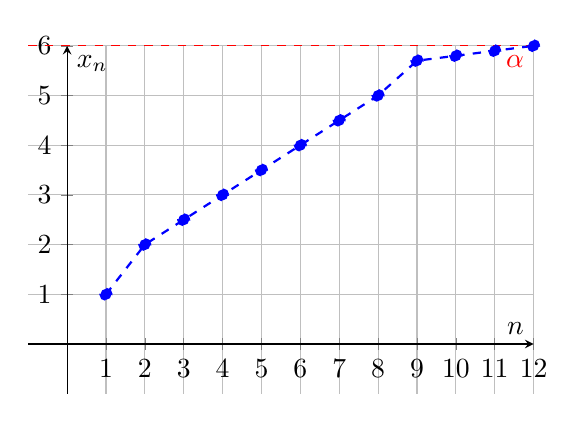
\begin{tikzpicture}
        \begin{axis}[
            axis lines = middle,
            xlabel = $n$,
            ylabel = {$x_n$},
            ymin = -1, ymax = 6,
            xmin = -1, xmax = 12,
            xtick={0,1,2,3,4,5,6,7,8,9,10,11,12},
            ytick={0,1,2,3,4,5,6},
            grid = both,
            width=8cm,
            height=6cm,
        ]
        \addplot[dashed, thick,
            color=blue,
            mark=*,
            mark options={fill=blue}
        ] coordinates {
            (1, 1)
            (2, 2)
            (3, 2.5)
            (4, 3)
            (5, 3.5)
            (6, 4)
            (7, 4.5)
            (8, 5)
            (9, 5.7)
            (10, 5.8)
            (11, 5.9)
            (12, 6)
        };
        \draw[dashed, red] (axis cs:-1,6) -- (axis cs:12,6) node[anchor=north east] {$\alpha$};
        \end{axis}
    \end{tikzpicture}
    \caption{An increasing and bounded sequence converging to its supremum $\alpha$}
\end{subfigure}
\begin{subfigure}{0.45\textwidth}
    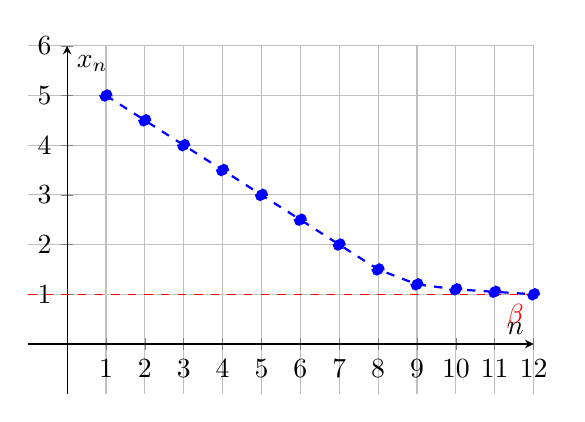
\begin{tikzpicture}
        \begin{axis}[
            axis lines = middle,
            xlabel = $n$,
            ylabel = {$x_n$},
            ymin = -1, ymax = 6,
            xmin = -1, xmax = 12,
            xtick={0,1,2,3,4,5,6,7,8,9,10,11,12},
            ytick={0,1,2,3,4,5,6},
            grid = both,
            width=8cm,
            height=6cm,
        ]
        \addplot[dashed, thick,
            color=blue,
            mark=*,
            mark options={fill=blue}
        ] coordinates {
            (1, 5)
            (2, 4.5)
            (3, 4)
            (4, 3.5)
            (5, 3)
            (6, 2.5)
            (7, 2)
            (8, 1.5)
            (9, 1.2)
            (10, 1.1)
            (11, 1.05)
            (12, 1)
        };
        \draw[dashed, red] (axis cs:-1,1) -- (axis cs:12,1) node[anchor=north east] {$\beta$};
        \end{axis}
    \end{tikzpicture}
    \caption{A decreasing and bounded sequence converging to its infimum $\beta$}
\end{subfigure}
\caption{Bounded monotonic sequences}
\end{figure}
\subsection{Subsequences}
\begin{mydefinition}
{Subsequence}
    A \underemphasise{subsequence} of a sequence $(x_n : n \in \N)$ is a sequence $(x_{n_k} : k \in \N)$ where $(n_k : k \in \N)$ is a strictly increasing sequence of natural numbers.
\end{mydefinition}

\begin{example}
    Consider the sequence $(x_n : n \in \N)$ defined as $x_n = (-1)^n$. The subsequence $(x_{2k} : k \in \N)$, where $n_k = 2k$, is given by:
    $$x_{2k} = (-1)^{2k} = 1$$
    \begin{figure}[H]
        \centering
        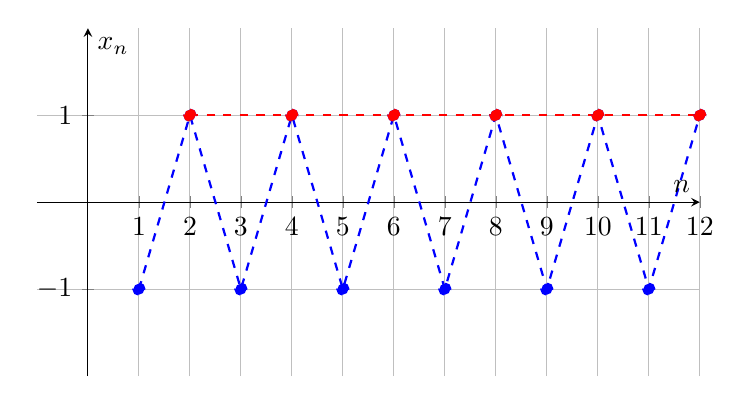
\begin{tikzpicture}
            \begin{axis}[
                axis lines = middle,
                xlabel = $n$,
                ylabel = {$x_n$},
                ymin = -2, ymax = 2,
                xmin = -1, xmax = 12,
                xtick={0,1,2,3,4,5,6,7,8,9,10,11,12},
                ytick={-1,0,1},
                grid = both,
                width=10cm,
                height=6cm,
            ]
            \addplot[dashed, thick,
                color=blue,
                mark=*,
                mark options={fill=blue}
            ] coordinates {
                (1, -1)
                (2, 1)
                (3, -1)
                (4, 1)
                (5, -1)
                (6, 1)
                (7, -1)
                (8, 1)
                (9, -1)
                (10, 1)
                (11, -1)
                (12, 1)
            };
            \addplot[dashed, thick,
                color=red,
                mark=*,
                mark options={fill=red}
            ] coordinates {
                (2, 1)
                (4, 1)
                (6, 1)
                (8, 1)
                (10, 1)
                (12, 1)
            };
            \end{axis}
        \end{tikzpicture}
        \caption{The subsequence $(x_{2k} : k \in \N)$ in red}
    \end{figure}
\end{example}
\begin{mytheorem}[Convergence of Subsequences]
    If a sequence $(x_n : n \in \N)$ converges to $L$, then all its subsequences converge to $L$.
\end{mytheorem}
\begin{proof}
    Let $(x_n : n \in \N)$ be a sequence that converges to $L$. Let $(x_{n_k} : k \in \N)$ be a subsequence of $(x_n : n \in \N)$. Then, by the definition of convergence, we have:
    $$\forall \epsilon > 0, \exists N \in \N: n > N \implies |x_n - L| < \epsilon$$
    Since $(n_k : k \in \N)$ is a strictly increasing sequence of natural numbers, we know that for all $k > N$, we have:
    $$n_k > N$$
    Therefore, we have:
    $$\forall k > N: |x_{n_k} - L| < \epsilon$$
    Hence, we conclude that all subsequences of a convergent sequence converge to the same limit.
\end{proof}
\begin{mynote}
    The converse of the above theorem is not true. That is, if all subsequences of a sequence converge to the same limit, it does not imply that the original sequence converges to that limit.
\end{mynote}
\begin{mytheorem}[Bolzano-Weierstrass Theorem]
    Every bounded sequence in $\R$ has a convergent subsequence.
\end{mytheorem}
\begin{proof}
    Let $M \in \R$ be such that the sequence $(x_n : n \in \N)$ is bounded by $M$. That is:
    $$\forall n \in \N, |x_n| \leq M$$
    Take the interval $I_0 = [-M, M]$. Now, we can divide this interval into two equal halves:
    $$I_1^1 = [-M, 0], I_1^2 = [0, M]$$
    At least one of these intervals must contain infinitely many terms of the sequence $(x_n : n \in \N)$. Let us denote this interval as $I_1$. Next, we can divide $I_1$ into two equal halves:
    $$I_2^1, I_2^2$$
    Again, at least one of these intervals must contain infinitely many terms of the sequence $(x_n : n \in \N)$. Let us denote this interval as $I_2$. Continuing this process, we can construct a sequence of nested intervals $(I_k : k \in \N)$ such that:
    \begin{enumerate}
        \item $I_{k+1} \subset I_k$ for all $k \in \N$
        \item The length of $I_k$ is $\frac{2M}{2^k}$
        \item Each interval $I_k$ contains infinitely many terms of the sequence $(x_n : n \in \N)$
    \end{enumerate}
    By the nested interval property, the intersection of all these intervals is non-empty. Therefore, there exists a point $c \in \R$ such that:
    $$c \in \bigcap_{k=1}^{\infty} I_k$$
    Since each interval $I_k$ contains infinitely many terms of the sequence $(x_n : n \in \N)$, we can extract a subsequence $(x_{n_k} : k \in \N)$ that converges to $c$. This completes the proof.
\end{proof}
\begin{mytheorem}[Every sequence has a monotonic subsequence]
    Every sequence in $\R$ has a monotonic subsequence.
\end{mytheorem}
\begin{proof}
    Let $(x_n : n \in \N)$ be a sequence in $\R$. We can construct a subsequence $(x_{n_k} : k \in \N)$ as follows:
    \begin{enumerate}
        \item Start with $n_1 = 1$.
        \item For each $k \geq 1$, choose $n_{k+1} > n_k$ such that $x_{n_{k+1}} \geq x_{n_k}$ if possible. If not, choose $n_{k+1} > n_k$ such that $x_{n_{k+1}} < x_{n_k}$.
    \end{enumerate}
    This process will yield either an increasing or decreasing subsequence. If at any step we cannot find a term that is greater than or equal to the previous term, we switch to finding a term that is less than the previous term, and vice versa. Since we can always find such terms in an infinite sequence, we will eventually construct a monotonic subsequence.
\end{proof}
\begin{mynote}
    The above theorem is useful in conjunction with the Bolzano-Weierstrass theorem to prove the convergence of subsequences.
\end{mynote}
\subsection{Cauchy Criterion and Cauchy Sequences}
\begin{mydefinition}{Cauchy Sequence}
    A sequence $(x_n : n \in \N)$ in $\R$ is said to be a \underemphasise{Cauchy sequence} if:
    $$\forall \epsilon > 0, \exists N \in \N: m,n > N \implies |x_n - x_m| < \epsilon$$
\end{mydefinition}
\begin{example}
    Consider the sequence $(x_n : n \in \N)$ defined as $x_n = \frac{1}{n}$. We will show that this sequence is a Cauchy sequence. \\
    Let $\epsilon > 0$. We need to find a natural number $N$ such that for all $m,n > N$, we have:
    $$|x_n - x_m| < \epsilon$$
    Without loss of generality, assume that $n > m$. Then, we have:
    $$|x_n - x_m| = \left|\frac{1}{n} - \frac{1}{m}\right| = \frac{|m - n|}{mn}$$
    Since $n > m$, we have $|m - n| = n - m$. Therefore, we can write:
    $$|x_n - x_m| = \frac{n - m}{mn}$$
    Now, since $m,n > N$, we have:
    $$mn > N^2$$
    Also, since $n - m < n$, we have:
    $$|x_n - x_m| < \frac{n}{N^2}$$
    To ensure that $|x_n - x_m| < \epsilon$, we can choose $N$ such that:
    $$\frac{n}{N^2} < \epsilon \implies N^2 > \frac{n}{\epsilon}$$
    Therefore, we can choose:
    $$N > \sqrt{\frac{n}{\epsilon}}$$
    Hence, we conclude that the sequence $(x_n : n \in \N)$ defined as $x_n = \frac{1}{n}$ is a Cauchy sequence.
\end{example}
\begin{mytheorem}[Cauchy Criterion]
    A sequence in $\R$ converges if and only if it is a Cauchy sequence.
\end{mytheorem}
\begin{proof}
    We prove both parts seperately. \\
    $(\Rightarrow)$ Let $(x_n : n \in \N)$ be a sequence that converges to $L$. Then, by the definition of convergence, we have:
    $$\forall \epsilon > 0, \exists N \in \N: n > N \implies |x_n - L| < \frac{\epsilon}{2}$$
    Let $m,n > N$. Then, we have:
    $$|x_n - x_m| = |(x_n - L) - (x_m - L)| \leq |x_n - L| + |x_m - L| < \frac{\epsilon}{2} + \frac{\epsilon}{2} = \epsilon$$
    Hence, we conclude that $(x_n : n \in \N)$ is a Cauchy sequence. \\
    $(\Leftarrow)$ Let $(x_n : n \in \N)$ be a Cauchy sequence. Then, by the definition of a Cauchy sequence, we have:
    $$\forall \epsilon > 0, \exists N \in \N: m,n > N \implies |x_n - x_m| < \epsilon$$
    Since $(x_n : n \in \N)$ is a Cauchy sequence, it is bounded. Therefore, by the Bolzano-Weierstrass theorem, it has a convergent subsequence $(x_{n_k} : k \in \N)$ that converges to some limit $L$. We need to show that the entire sequence $(x_n : n \in \N)$ converges to $L$. \\
    Let $\epsilon > 0$. Then, by the definition of convergence of the subsequence, we have:
    $$\exists K \in \N: k > K \implies |x_{n_k} - L| < \frac{\epsilon}{2}$$
    Also, since $(x_n : n \in \N)$ is a Cauchy sequence, we have:
    $$\exists N' \in \N: m,n > N' \implies |x_n - x_m| < \frac{\epsilon}{2}$$
    Let $N = \max(N', n_K)$. Then, for all $n > N$, we have:
    $$|x_n - L| = |(x_n - x_{n_K}) + (x_{n_K} - L)| \leq |x_n - x_{n_K}| + |x_{n_K} - L| < \frac{\epsilon}{2} + \frac{\epsilon}{2} = \epsilon$$
    Hence, we conclude that $(x_n : n \in \N)$ converges to $L$.
\end{proof}
\begin{mynote}
Why is the above criterion only valid in $\R$ and not in general for any metric space? \\
    The Cauchy criterion relies on the completeness property of the real numbers. A metric space is said to be complete if every Cauchy sequence in that space converges to a limit that is also within that space. The real numbers $\R$ are complete, which is why the Cauchy criterion holds true for sequences in $\R$. However, not all metric spaces are complete. For example, the rational numbers $\Q$ are not complete because there exist Cauchy sequences of rational numbers that converge to irrational limits, which are not in $\Q$. Therefore, the Cauchy criterion may not hold in such spaces.
\end{mynote}
\begin{mytheorem}[A Cauchy sequence is bounded]
    Every Cauchy sequence in $\R$ is bounded.
\end{mytheorem}
\begin{proof}
    Let $(x_n : n \in \N)$ be a Cauchy sequence. Then, by the definition of a Cauchy sequence, we have:
    $$\forall \epsilon > 0, \exists N \in \N: m,n > N \implies |x_n - x_m| < \epsilon$$
    Let $\epsilon = 1$. Then, there exists a natural number $N$ such that for all $m,n > N$, we have:
    $$|x_n - x_m| < 1$$
    In particular, for all $n > N$, we have:
    $$|x_n - x_{N+1}| < 1 \implies |x_n| < |x_{N+1}| + 1$$
    Let $M = \max\{|x_1|, |x_2|, \ldots, |x_N|, |x_{N+1}| + 1\}$. Then, we have:
    $$\forall n \in \N, |x_n| \leq M$$
    Hence, we conclude that every Cauchy sequence in $\R$ is bounded.
\end{proof}
\subsection{Limit Superior and Limit Inferior}
\begin{mydefinition}{Limit Superior and Limit Inferior}
    Let $(x_n : n \in \N)$ be a sequence in $\R$. The \underemphasise{limit superior} (or \underemphasise{lim sup}) of the sequence is defined as:
    $$\limsup_{n \to \infty} x_n = \lim_{n \to \infty} (\sup\{x_k : k \geq n\})$$
    The \underemphasise{limit inferior} (or \underemphasise{lim inf}) of the sequence is defined as:
    $$\liminf_{n \to \infty} x_n = \lim_{n \to \infty} (\inf\{x_k : k \geq n\})$$
\end{mydefinition}
\begin{example}
    Consider the sequence $(x_n : n \in \N)$ defined as $x_n = (-1)^n + \frac{1}{n}$. We will find the limit superior and limit inferior of this sequence. \\
    First, we note that the sequence oscillates between values close to 1 and -1 as $n$ increases. Specifically, for even $n$, we have:
    $$x_{2k} = 1 + \frac{1}{2k}$$
    and for odd $n$, we have:
    $$x_{2k+1} = -1 + \frac{1}{2k+1}$$
    Now, we can find the limit superior:
    $$\limsup_{n \to \infty} x_n = \lim_{n \to \infty} (\sup\{x_k : k \geq n\})$$
    As $n$ increases, the supremum of the set $\{x_k : k \geq n\}$ approaches 1. Therefore, we have:
    $$\limsup_{n \to \infty} x_n = 1$$
    Next, we can find the limit inferior:
    $$\liminf_{n \to \infty} x_n = \lim_{n \to \infty} (\inf\{x_k : k \geq n\})$$
    As $n$ increases, the infimum of the set $\{x_k : k \geq n\}$ approaches -1. Therefore, we have:
    $$\liminf_{n \to \infty} x_n = -1$$
    Hence, we conclude that for the sequence $(x_n : n \in \N)$ defined as $x_n = (-1)^n + \frac{1}{n}$, the limit superior is 1 and the limit inferior is -1.
\end{example}
\begin{figure}[H]
    \centering
    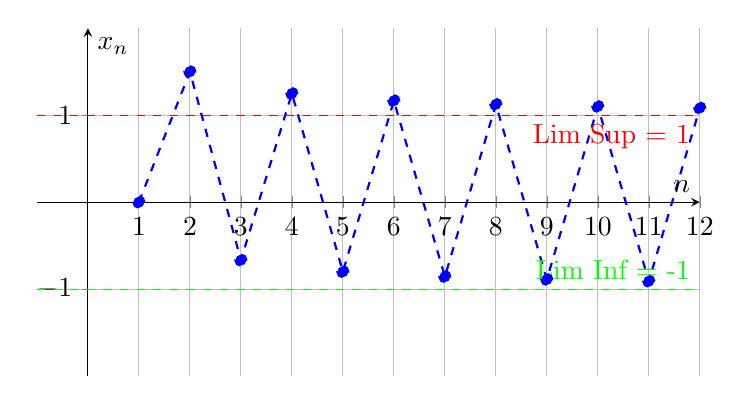
\begin{tikzpicture}
        \begin{axis}[
            axis lines = middle,
            xlabel = $n$,
            ylabel = {$x_n$},
            ymin = -2, ymax = 2,
            xmin = -1, xmax = 12,
            xtick={0,1,2,3,4,5,6,7,8,9,10,11,12},
            ytick={-1,0,1},
            grid = both,
            width=10cm,
            height=6cm,
        ]
        \addplot[dashed, thick,
            color=blue,
            mark=*,
            mark options={fill=blue}
        ] coordinates {
            (1, 0)
            (2, 1.5)
            (3, -0.6667)
            (4, 1.25)
            (5, -0.8)
            (6, 1.1667)
            (7, -0.8571)
            (8, 1.125)
            (9, -0.8889)
            (10, 1.1)
            (11, -0.9091)
            (12, 1.0833)
        };
        \draw[dashed, red] (axis cs:-1,1) -- (axis cs:12,1) node[anchor=north east] {Lim Sup = 1};
        \draw[dashed, green] (axis cs:-1,-1) -- (axis cs:12,-1) node[anchor=south east] {Lim Inf = -1};
        \end{axis}
    \end{tikzpicture}
    \caption{Limit Superior and Limit Inferior of the sequence $x_n = (-1)^n + \frac{1}{n}$}
\end{figure}
\begin{mynote}
    What is the significance of limit superior and limit inferior? \\
    The limit superior and limit inferior provide a way to analyze the behavior of sequences that do not converge in the traditional sense. They help us understand the "bounds" within which the sequence oscillates. The limit superior gives us the largest value that the sequence approaches infinitely often, while the limit inferior gives us the smallest value that the sequence approaches infinitely often. This is particularly useful for sequences that oscillate or have multiple accumulation points. \\ \\
    How are limsup and liminf different from the usual limit of a sequence? \\
    The usual limit of a sequence, if it exists, is a single value that the sequence approaches as $n$ goes to infinity. In contrast, the limit superior and limit inferior can exist even when the usual limit does not. They provide a way to describe the "envelope" of the sequence's behavior, capturing the extreme values that the sequence approaches infinitely often, rather than a single convergent value.
\end{mynote}

\begin{mytheorem}[Equality of LimSup and LimInf for Convergent Sequences]
    If and only if a sequence $(x_n : n \in \N)$ converges to $L$, then:
    $$\limsup_{n \to \infty} x_n = \liminf_{n \to \infty} x_n = L$$
\end{mytheorem}
\begin{proof}
    We prove both parts seperately. \\
    $(\Rightarrow)$ Let $(x_n : n \in \N)$ be a sequence that converges to $L$. Then, by the definition of convergence, we have:
    $$\forall \epsilon > 0, \exists N \in \N: n > N \implies |x_n - L| < \epsilon$$
    This implies that for all $n > N$, we have:
    $$L - \epsilon < x_n < L + \epsilon$$
    Therefore, we can write:
    $$\sup\{x_k : k \geq n\} < L + \epsilon$$
    $$\inf\{x_k : k \geq n\} > L - \epsilon$$
    Taking the limit as $n$ approaches infinity, we have:
    $$\limsup_{n \to \infty} x_n \leq L + \epsilon$$
    $$\liminf_{n \to \infty} x_n \geq L - \epsilon$$
    Since $\epsilon$ is arbitrary, we conclude that:
    $$\limsup_{n \to \infty} x_n = L$$
    $$\liminf_{n \to \infty} x_n = L$$
    $(\Leftarrow)$ Let $(x_n : n \in \N)$ be a sequence such that:
    $$\limsup_{n \to \infty} x_n = L$$
    $$\liminf_{n \to \infty} x_n = L$$
    We need to show that $(x_n : n \in \N)$ converges to $L$. Let $\epsilon > 0$. Then, by the definitions of limit superior and limit inferior, we have:
    $$\exists N_1 \in \N: n > N_1 \implies \sup\{x_k : k \geq n\} < L + \epsilon$$
    $$\exists N_2 in \N: n > N_2 \implies \inf\{x_k : k \geq n\} > L - \epsilon$$
    Let $N = \max(N_1, N_2)$. Then, for all $n > N$, we have:
    $$L - \epsilon < x_n < L + \epsilon$$
    Therefore, we have:
    $$|x_n - L| < \epsilon$$
    Hence, we conclude that $(x_n : n \in \N)$ converges to $L$.
\end{proof}
















\end{document}
